\chapter{Experimental results}
In this chapter, I will present the experimental results.
First, the methodology that I used to construct the sensor software update benchmarks are addressed.
Then, I divided the experimental results into two parts,
the data collected before code dissemination and the data collected after code dissemination.
The former part compares the trade-off between the generated script size and the code performance for both general purpose and DSP applications.
The latter part compares the network traffic and time consumption between the proposed protocol with
the other existing schemes.

\section{Benchmarks}
Because the software update management is a new problem to study
in the wireless embedded system community, there is no existing
update benchmarks available to evaluate the performance gain
of my proposed framework.
Therefore, I built a sensor software update benchmark suite
which covers the software update cases for both general purpose
applications and DSP applications that run on the wireless
embedded devices.

The base benchmarks are from the general purpose
sensing applications included in TinyOS~\cite{tinyos}--
an open-source operating system designed for wireless embedded
sensor networks, CryptoLib -- the encryption library, and the DSP applications included in 
DSPstone~\cite{dspstone} benchmark suite. 
Upon the base benchmark, I created the pairing update benchmark
using three different techniques and categorized them based on the update levels.

\subsection{Update levels}
There are three update levels according to their
impact on code structures: 
(a) low level updates, which are made to local basic blocks; 
(b) medium level updates, which include changes in a large
function or across several functions, but still preserve the overall
structure of the original code; 
(c) high level updates, which significantly
change the code structure. Frequent updates such as code fixes and
sensor reconfigurations are mainly low or medium level changes, while
replacing the application with a new one introduces medium to high level
changes. 

\subsection{Real update benchmarks (real-benches)}
One application may have multiple versions that exist in the
base benchmarks to add new features of fix bugs that exist 
in the old version.
For example, TinyOS-1.x has over 15 versions, and in each release
the enclosed applications may be updated.
Updates made to the applications vary from adding one statement
to completely reconstructing the code.
As the proposed software update management framework targets
at low or medium level code updates, I selected the proper sized real code
update cases that exist in the base benchmarks as the real update
benchmarks.
These real update benchmarks will show the real update patterns
for the applications running on wireless embedded devices and
become the base of generating the other two update benchmarks.

\subsubsection{General purpose application update benchmark}
Figure~\ref{fdeluge.src} shows one real update case of the general purpose
software.
The function unit Deluge~\cite{deluge}, a reliable code dissemination protocol
enclosed in TinyOS is studied.I studied updates of Deluge from TinyOS version 1.52 
to version 1.58. The update details are shown in the figure.

\begin{figure}[htbp]
\begin{center}
\begin{small}
\begin{tabular}{||p{0.5in}|p{1in}|p{0.6in}|p{3.5in}||} \hline

Case\# & Versions & Update Level & Update details \\ \hline \hline

R-G-1 &  ${1.52 \Rightarrow 1.53}$ & Low & Add one statement to reset one variable. \\ \hline
R-G-2 &  ${1.53 \Rightarrow 1.54}$ & High & Add one variable, and related statements to
	update this variable when necessary. One statement is updated to use this variable instead. \\ \hline
R-G-3 &  ${1.54 \Rightarrow 1.55}$ & Medium & Modify the condition of two ``if'' statements. \\ \hline
R-G-4 &  ${1.55 \Rightarrow 1.56}$ & High & Move one function. Add one ``if'' statement to reset 
	one variable when it's invalid, and all the other four related variables. \\ \hline
R-G-5 &  ${1.56 \Rightarrow 1.57}$ & Medium & Move two ``memcpy'' statements to be next to the relative ``if'' statements. \\ \hline
R-G-6 &  ${1.57 \Rightarrow 1.58}$ & High & Modify the condition of two ``if'' statements. Add two ``for'' loops. Remove two statements. \\ \hline

\end{tabular}
\end{small}
\end{center}
\caption{Real general purpose application update benchmark.}
\label{fdeluge.src}
\end{figure}

\subsubsection{DSP application update benchmark}

\begin{figure}[htdp]
\begin{small}
\begin{center}
\begin{tabular}{||p{0.5in}|p{1.5in}|p{0.6in}|p{3.5in}||}
\hline
Case\#  &  Function & Update & Description \\
 & \& Versions &Level&\\
\hline\hline
R-D-1 &  matrix1.c$\Rightarrow$matrix2.c& medium & Move two iterations out of the loop.\\
\hline
R-D-2 &  speed\_control 1 $\Rightarrow$2 & medium &Seven temporary variables are introduced to hold the value of the comparison results.\\
\hline
R-D-3 & speed\_control 2 $\Rightarrow$3 &high &  Multiple global variables are combined into a structure. The reference to the variables are changed due to this change.\\
\hline
\end{tabular}
\end{center}
\caption{Real DSP application update benchmark. }
\label{dsp-bench}
\end{small}
\end{figure}
For the DSP applications, I selected the matrix multiplication function {\it matrix.c} and one function in the ADPCM standard implement {\it speed\_control} as the real DSP update benchmarks. More information can be found in Figure~\ref{dsp-bench}. 



\subsection{Manually generated update benchmarks (man-benches)}
Software updates are manually inserted to the base benchmarks to create the
manually generated update benchmarks.
The manual inserted code is designed to cover all possible code update circumstances
including variable insertion/deletion, 
instructions insertion/deletion/update inside and outside loops, and the control flow
insertion/deletion/update.
\begin{figure}[htbp]
\centering
\begin{small}
\begin{tabular}{||p{1in}|p{0.5in}|p{4in}||} 
\hline
Base  & Source & Details \\ 
benchmark & & \\\hline  \hline

Blink & TinyOS & It starts a 1Hz timer and toggles the red
LED every time it fires. \\ \hline

CntToLeds & TinyOS & It maintains a counter on a 4Hz timer and
displays the lowest three bits of the counter value. The red LED is
the least significant of the bits, while the yellow is the most
significant. \\ \hline

CntToRfm & TinyOS & It maintains a counter on a 4Hz timer and sends
out the value of the counter in an IntMsg AM packet on each
increment. \\ \hline

CntToLeds AndRfm & TinyOS & It maintains a counter on a 4Hz timer; it
combines the tasks performed by CntToRfm and CntToLeds. \\ \hline

AES & Crypto Lib & It encrypts a given 128 bit input buffer using AES
algorithm. I select the encryption code in the experiment.\\ \hline \hline

Deluge & TinyOS & The mulithop code dissemination protocol in TinyOS. I tracked its continuous updates in different TinyOS versions as a real life case study. \\ \hline
\end{tabular}
\end{small}
\caption{Base benchmarks for general purpose applications.}
\label{fbench}
\end{figure}


\subsubsection{General purpose application update benchmark}
The TinyOS application shown in Figure~\ref{fbench} are selected as the base benchmarks
to create the manaually generated general purpose software update benchmark.


Figure \ref{fbench.chg1} summarizes the synthetic updates made to these
benchmarks. The updates vary from low level, through medium level, to high level changes.

\begin{figure}[htbp]
\centering
\begin{small}
\begin{tabular}{||p{0.6in}|p{1in}|p{0.5in}|p{3.5in}||} \hline
Case \# & Function & Update Level & Update details \\ \hline \hline

M-G-1 & CntToLeds &Low & Change the color of blink. \\ \hline

M-G-2 & Blink &Low & Insert one local variable and one use in
run\_next\_task. \\ \hline

M-G-3 & AES& Low & Insert one local variable and use it within the
loop in aes\_encrypt. \\ \hline

M-G-4 & AES & Low & Change one instruction in aes\_encrypt. \\ \hline

M-G-5 & AES & Low & Insert a local variable in aes\_encrypt and use it
twice --- within and outside the loop. \\ \hline

M-G-6 & Blink &Low &Add a new parameter in TOSH\_run\_task. \\ \hline

M-G-7 & CntToLeds & Medium & Insert three variables and their uses; \\
\hline

M-G-8 & CntToRfm & Medium & Insert a global variable and use in three
different functions. \\ \hline

M-G-9 & CntToRfm & Medium & Insert a local variable and use it several
times in TOSH\_run\_next\_task function. \\ \hline

M-G-10 & Blink&Medium & Insert a global variable and use it in a new
if/then branch in TOSH\_run\_next\_task function. \\ \hline

M-G-11 & Blink & Medium & Add an else branch for an if statement in Timer\_HandleFire. \\ \hline

M-G-12 & CntToRfms $\Rightarrow$ CntToLedsRfm &high & Change the application from CntToRfms to CntToLedsRfm \\ \hline 

M-G-13* &CntToLeds$\Rightarrow$ CntToRfms &high & Change the application from CntToLeds to CntToRfms. \\ \hline 

M-G-14 & AES & Medium & Add two and remove one local variables in function invShiftRows().
\\ \hline
M-G-15 & AES & Medium & Add one and remove two local variables in function invShiftRows().
\\ \hline

M-G-16 & AES & Medium & Add one local variable in function invShiftRows() and add a four element array in function invMixSubColumns().\\ \hline
M-G-17 & AES & Medium & Remove one local variable in function invShiftRows() and remove a four element array in function invMixSubColumns().\\ \hline


M-G-18 & AES & High & Remove one and add two local variables in function invShiftRows(). Remove two and add four local variables in function invMixSubColumns().\\ \hline
M-G-19 & AES & High & Add one and remove two local variables in function invShiftRows(). Add two and remove four local variables in function invMixSubColumns().\\ \hline

\multicolumn{4}{l}{*: The experimental results of this case are shown in the text instead of the graphs to make}\\
\multicolumn{4}{l}{the graphs more proportionally precise.}\\
\end{tabular}
\end{small}
\caption{Manually generated general purpose application update benchmark.}
\label{fbench.chg1}
\end{figure}


\subsubsection{DSP application update benchmark}
For the DSP applications, I inserted/deleted code to create/remove the variable interferences to the DSP base benchmarks, such as the matrix multiplication function {\it matrix.c} and one function in the ADPCM standard implement {\it speed\_control} as the real DSP update benchmarks. 
The detailed benchmarks are listed in Figure~\ref{dsp-manual}. 

\begin{figure}[htdp]
\begin{small}

\begin{center}
\begin{tabular}{||p{0.5in}|p{0.6in}|p{1.2in}|p{3.5in}||}
\hline
Test &   Function & Update &Description \\
Case & & Level&\\
\hline\hline
M-D-1  & verify.c& Low & Update \textbf{one basic block}  to create
the interference between two variables that are \textbf{not coalesced} 
in the original version.\\
\hline
M-D-2  & verify.c& medium & Update \textbf{one basic block} to create
the interference between three variables that are \textbf{coalesced}
in the original version. \\
\hline
M-D-3  & verify.c& medium & Expand the live ranges of three variables to
\textbf{cross basic blocks}. \\
\hline
M-D-4   & matrix1.c& medium & Shrink the live range of the one variable and
Expand the live range of another variable within on basic block.  \textbf{ Over
ten interferences} are updated.\\
\hline
M-D-5 & matrix1.c& medium  & Shrink the live ranges of the two variables and
Expand the live ranges of another two variables within on basic block.
 \textbf{Over ten interferences} are updated.\\
\hline
\end{tabular}
\end{center}
\caption{Manually DSP application update benchmark.}
\label{dsp-manual}
\end{small}
\vspace{-0.1in}
\end{figure}%

\subsection{Automatically generated update benchmarks (auto-benches)}
In order to study more general cases and to evaluate the compiler performance,
I also wrote a tool to generate the update benchmarks automatically.

\subsubsection{General purpose application update benchmark}
For general purpose application study, 
the generated test cases are used to evaluate the compilation time of the update-conscious compilation schemes. The compilation time here depends on the complexity of the
ILP problem created by update-conscious compiler.  
Because the number of decision variables, constrains and the complexity of
the objective goal all affect the problem complexity, one source level modification may create problems with
quite different complexity levels depending on the type of the modification
and the place where it is made. 
Thus, instead of modifying the source code, I created the benchmarks
by modifying the intermediate representations directly.
Random intermediate representation statements are inserted to or removed from the 
intermediate representation of the base benchmark.
Given the number of intermediate representation statements to be modified,
I created multiple cases to show the bound of how that affects to the problem complexity.

\subsubsection{DSP application update benchmark}
For DSP application study, the automatically generated test cases are used to evaluate
the compilation performance, including the patch script size deduction and
the run-time execution overhead, to cover broader cases.
Because the direct factors are the memory access sequence and the interference
between each pair of variables, I created the automatically generated 
benchmarks by directly modifying these two factors.

\subsubsection{Methodology used to generate the auto-benches}
Although I built the auto-benches for general purpose applications and DSP applications
based on different input, the methodology used to generate the auto-benches is the same.
For the general purpose applications, the IRs of a base application act as the input of
the auto-bench generator. 
For the DSP applications, the access sequence as well as the interferences
are the inputs instead.
To simply the description, let us define one input statement as one IR statement for the first type of input, 
one variable in the access sequence or one interference between
two variables for second type of input.

For a given input, the point between each two statements and the point after the last statement are called an update point.
Given the update percentage, the number of statements that need to be updated is fixed
for one base application.
A random set of the update points will be selected for updates according to this number.
Several update options can be made at each update point, such as inserting a new statement,
removing the prior statement or updating the prior statement.
A random decision will be made at each update point to create a change.

Several trails are run to create a set of the auto-bench for a given update percentage.
There may be some cases that are not semantically correct.
For example, the updates that are randomly inserted to the IRs of a general purpose
application may not make sensor so that the ILP cannot compute a valid result.
These cases are removed from the set and a new valid case will be generated to replace it.

\section{Pre-dissemination performance evaluation}
I implemented my proposed update-conscious schemes, including the register allocation
(UCC-RA), data allocation (UCC-DA) and the integrated scheme.
I compared the compiler performance between the update-conscious compiler and 
the GNC C compiler (GCC-RA and GCC-DA representatively). 
The UCC-RA scheme trades off the run time code performance for a smaller update script
that results in a lower transmission energy.

In this
section, I will discuss my experimental settings and present the results
on code quality, energy efficiency, and compilation time.

\subsection{General purpose software update using UCC-RA}\label{exper-ra}

In order to compare the performance of the proposed update-conscious compilation register
allocation scheme (UCC-RA) with GCC-RA, I used the manual generated general purpose 
benchmarks (M-G-1 $\sim$ M-G-13) list in
Figure~\ref{fbench.chg1} to generate the binary images and further the patch scripts.
Then, I used automatically generated general purpose benchmarks to study the
problem complexity and compilation time.
\subsubsection{Settings}

I simulated a sensor network that consists of Mica2 mote nodes
\cite{mica2-power} running TinyOS~\cite{tinyos},  an open source
operating system designed for WSNs.  The processor that Mica2
(MPR400CB model) uses is the AMTEL AVR micro controller ---
ATmega128L~\cite{atmega128L}.  

To compile the code for Mica2, I chose {\tt ncc}, the NesC compiler
included in TinyOS release, and {\tt avr-gcc}, the GNU C compiler
(GCC) re-targeted for AMTEL AVR micro controllers. I used {\tt -O3}
option to compile the code and ensured the code fit in the sensor
storage (i.e. I considered {\tt -Os} option as well).  I used the
default register allocator of the {\tt gcc/avr-gcc}, for using the new
iterative graph allocator (with the option {\tt -fnew-ra}) would give
similar results.

I selected {\tt Avrora}, an instruction-level sensor network
simulator, to collect the execution cycles of the code before and
after compiling the updated code with UCC and GCC (the accuracy of the
simulator has been reported in prior work~\cite{avrora}). I then
integrated the energy model and execution profiles to study the energy
consumption tradeoffs with different compilation approaches.

The update script generator is implemented over Diffutils~\cite{diff}
to format the output in the proposed format.



\subsubsection{The generate script size}
Figure \ref{fbench.chg1} summarizes the synthetic updates that I made to the
benchmarks. The updates vary from low level, through medium level, to high level changes,
as described below:
\begin{itemize}
\itemsep 0pt
\item
The low and medium level test cases cover a wide range of changes
including constant changes, variable changes, parameter changes,
instruction changes, and control flow changes. More complex updates
may require one or more such changes.

\item 
Complex updates tend to create changes over many functions, though
most of these test cases impact only one function.  To fairly evaluate
the UCC-RA and decouple its impact from data allocation and code
layout, I only report the changes in the functions that are directly
affected (rather than, for instance, code shifting due to
expansion/shrinkage of neighbor functions).  In addition, I observed
minimal inter-procedural correlation. For example, the same global
variable can be assigned with different registers in different
functions.  Therefore the overall impact of high level updates can be
estimated by summarizing the changes in simple updates.

\item
I evaluated the code changes using $\textit{Diff}_{script\_size}$, the
size of the update scripts that are used to change the old binaries to the
new ones. 

%We use $Diff_{bytes}$ instead of the edit script size since
%the latter is dependent on other factors such as packing or grouping
%the code differences in different manners. For example, assume we have
%two scripts which contain 10 and 11 edit primitives respectively. If
%one transmission packet can pack 10 edit primitives, the script with
%11 primitives needs two packets --- a 100\% increase from the one with
%10 primitives in terms of the packet number.
\end{itemize}


I first conducted experiments to compare the generated script size
between UCC-RA and GCC-RA.  For GCC-RA, I manually find the best
match between the new and the old binaries. This is the lower bound of
existing {\em binary-diff-}based code dissemination algorithms
\cite{flink,related:script}. That is, I compared my results against the best possible
implementation of existing update-unconscious approaches
\cite{flink,related:script}. 

\vspace{0.2in}
\begin{figure}[htbp]
\centering
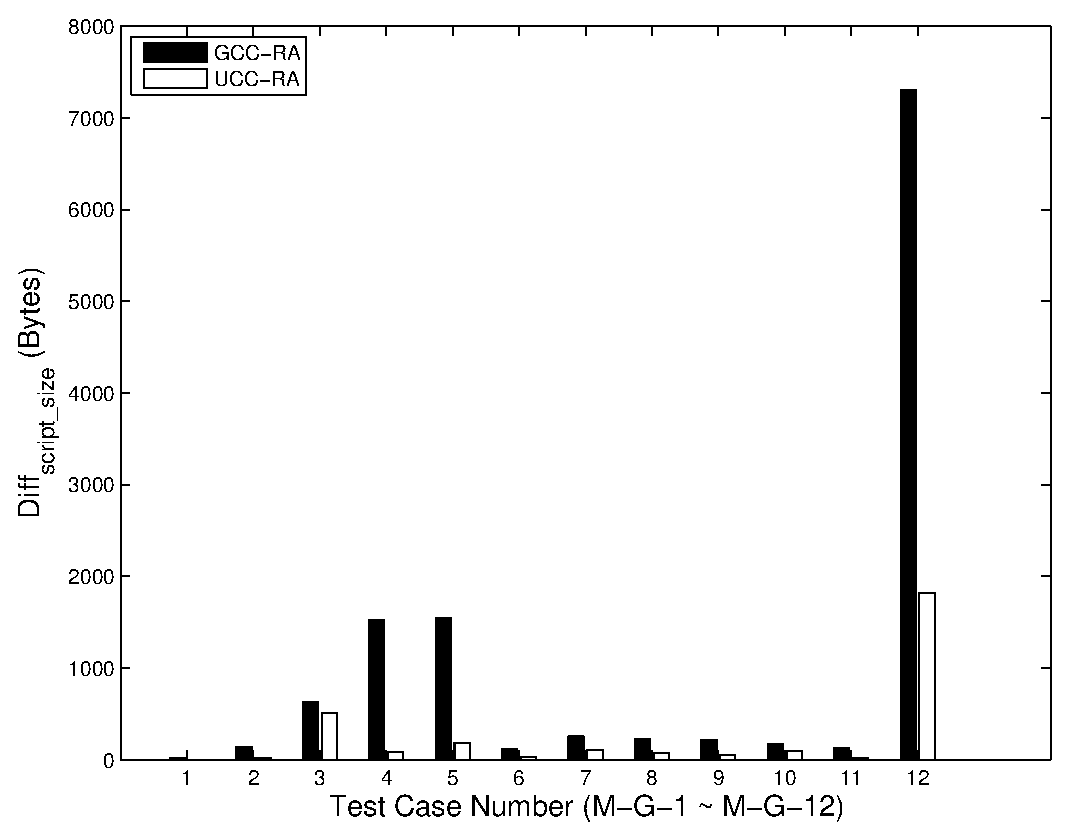
\includegraphics[scale=0.6]{figures/upd.eps}
\caption{Script size comparison between UCC-RA and GCC-RA.}
\label{fexp.upd}
\end{figure}

Figure \ref{fexp.upd} shows the results, in $\textit{Diff}_{script\_size}$, for update
test cases M-G-1 $\sim$ M-G-12.  As I can see, UCC-RA greatly reduces the code
difference as it effectively localizes the code changes --- the
majority of the code can be kept the same.  On the contrary, GCC-RA
may generate only local changes (test case M-G-1), but may also propagate local
changes to a much larger range (test case M-G-4).

I then studied the two high level changes. Test case 12 introduces
several new functions most of which are small {\em inline}
functions. They disturb the register selection in a large function and
introduce significant number of differences, which are seen when using
GCC-RA. Fortunately, those differences are minimized in UCC-RA.
Test case M-G-13 represents another type of high level
changes, the application {\tt CntToLeds} is quite different from
{\tt CntToRfms}.  The former has 828 instructions while the latter has
4351 instructions. It is an expensive update since all new instructions
and functions have to be disseminated across the network. There is
some code similarity due to the fact that applications in the same
TinyOS environment follow a generic structure.  GCC-RA can reuse 422
instructions and need to update 3929 instructions. UCC-RA can reuse 63
more instructions, which represents an increase of 15\% from GCC-RA,
and accounts for about 7.6\% of the old code ({\tt CntToLeds}).

\subsubsection{The generated code quality}\label{ucc-ra-code}
Next, I compared the code quality resulting from different
algorithms. The code quality is quantified using $\textit{Diff}_{cycle}$, the
changes in execution cycles between the old and new version of the
binary. This metric also indicates the slowdown in execution time
after applying update-conscious compilation.

\begin{figure}[htbp]
\centering
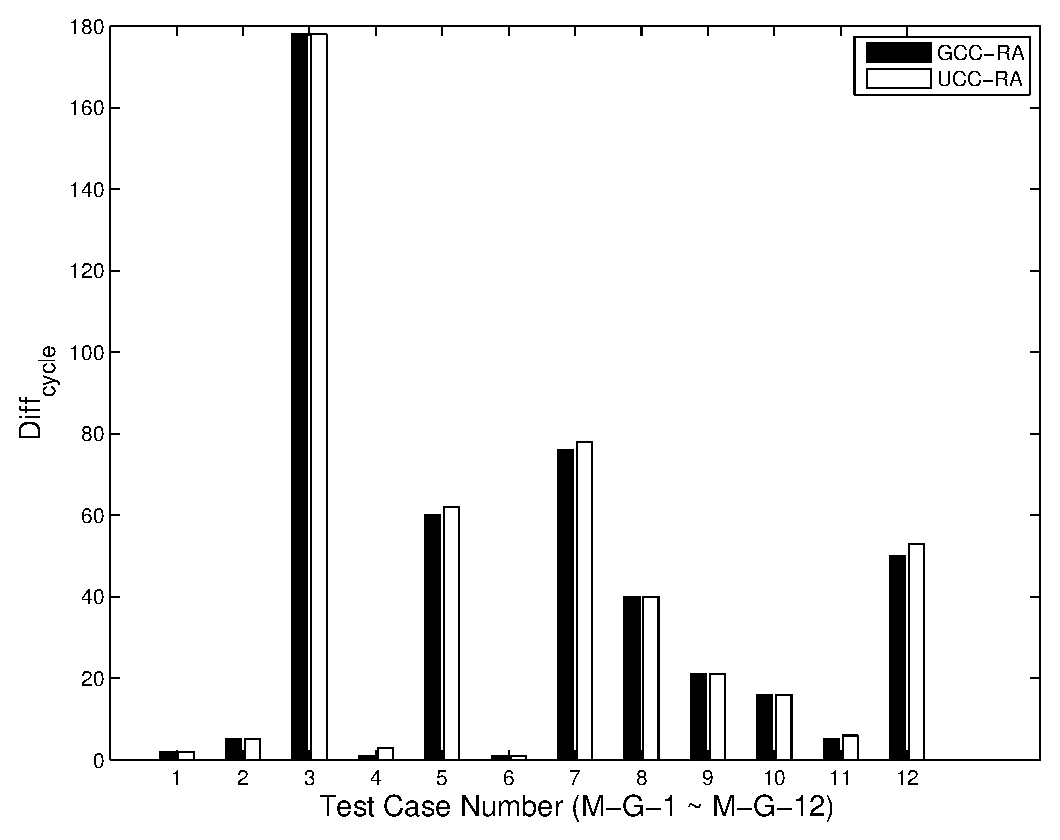
\includegraphics[scale=0.6]{figures/prof.eps}
\caption{Code quality comparison between UCC-RA and GCC-RA.}
\label{fexp.perf}
\end{figure}

Figure \ref{fexp.perf} shows the results for test case M-G-1 $\sim$ M-G-12. In
most of these cases, UCC-RA and GCC-RA have the same $\textit{Diff}_{cycle}$,
i.e. they have the same code quality. This is because both of them can
find free registers to use, and no extra spill code need to be
generated. Thus, register conflicts are small.  In some cases, e.g.,
test case M-G-12, UCC-RA inserts three {\tt mov} instructions since by
doing so, it can save 406 instruction updates and achieve overall
energy efficiency.

The slowdown from applying UCC-RA is negligible in nearly
all cases. For example, the three cycles introduced by UCC-RA in test
case M-G-12 accounts for less than 0.01\% of 244K cycles --- the total
number of cycles per single run for the application {\tt CntToRfm}. We
study its energy consumption over a long period after many
invocations, in the next section.

For test case M-G-13, UCC-RA only uses the preferred register tag as hint
when selecting registers. It has the same code quality as the one
generated by GCC-RA.

\subsubsection{The energy savings}
%To study the energy consumption in more detail, we conducted the
%experiment to compare the energy consumption using the above two
%register allocation algorithms.
The energy savings per update are calculated as follows. I first
compute $\textit{Diff}_{energy}$ (defined below), the energy consumption
difference (per single run) before and after the code update. It
incorporates the energy consumed in both data transmission and
instruction execution. Second, I compute the energy savings per
update for GCC-RA and UCC-RA respectively.

\begin{small}
\begin{eqnarray}
\textit{Diff}_{energy} =
\textit{Diff}_{script\_size} \times E_{trans} + \textit{Diff}_{cycle} \times E_{exe} \times Cnt \\
Energy Savings =
\textit{Diff}_{energy}^{GCC-RA} - \textit{Diff}_{energy}^{UCC-RA}
\end{eqnarray}
\end{small}

\noindent
where $Cnt$ is the total number of times that the code may be executed
before it retires. A code retires when either it is overwritten by
a later update or the sensor node has consumed all its battery energy
and dies.

Figure \ref{fexp.energy} plots the the energy savings of UCC-RA over
GCC-RA as a function of $Cnt$, which is projected from the execution
profiles and the code update frequency. Code fragments that reside in
a loop, or retire after a long time, have larger $Cnt$s than
others. From the figure, I can see that when UCC-RA and GCC-RA
generate the same quality code (same \textit{Diff$_{cycle}$}, such as for test
case 1), the energy savings are independent of $Cnt$. The savings
mainly come from the reduced transmission energy. The larger number
of instructions I reduce from GCC-RA, the less data I need to
transmit, and the more savings I gain from UCC-RA.

\begin{figure}[htbp]
\centering
\includegraphics[scale=0.45]{figures/energy.eps}
\caption{The energy savings per update for general purpose applications.}
\label{fexp.energy}
\end{figure}

When the code generated from UCC-RA runs slightly slower than that from GCC-RA (e.g., test case M-G-12), extra energy will be consumed in instruction execution. This can diminish the transmission energy savings when the code is executed very frequently. Therefore, UCC-RA adaptively inserts {\tt mov} instructions according to execution profiles and update frequency. A large $Cnt$ would disable the insertion such that UCC-RA and GCC-RA have the same energy consumption in the worst case. For example, UCC-RA falls back to take the GCC-RA's decision when the modified in code test case 12 is projected to execute more than 10$^7$ times.
%because of the diminishing energy gain.



\subsubsection{The problem complexity and compilation time}
For a given program, automatically generated general purpose software update
benchmarks are used to evaluate the ILP problem
complexity which is affected by the number of constrains and the number of
decision variables and the compilation time spent solving the ILP problem.

Since the ILP problem is more complex to solve when the number of
instructions and variables increase, I discuss the problem complexity
in this section. Figure~\ref{fexp.inst.con} plots the number of
constraints as a function of instruction number. I can see that the
number of constraints increases almost linearly with the number of IR
instructions. I plot the number of iterations that the LP\_solve
\cite{lpsolve} requires as a function of (the number of variables
$\times$ the number of IR instructions) in Figure~\ref{fexp.iter.con}.
\begin{figure}[htbp]
\centering
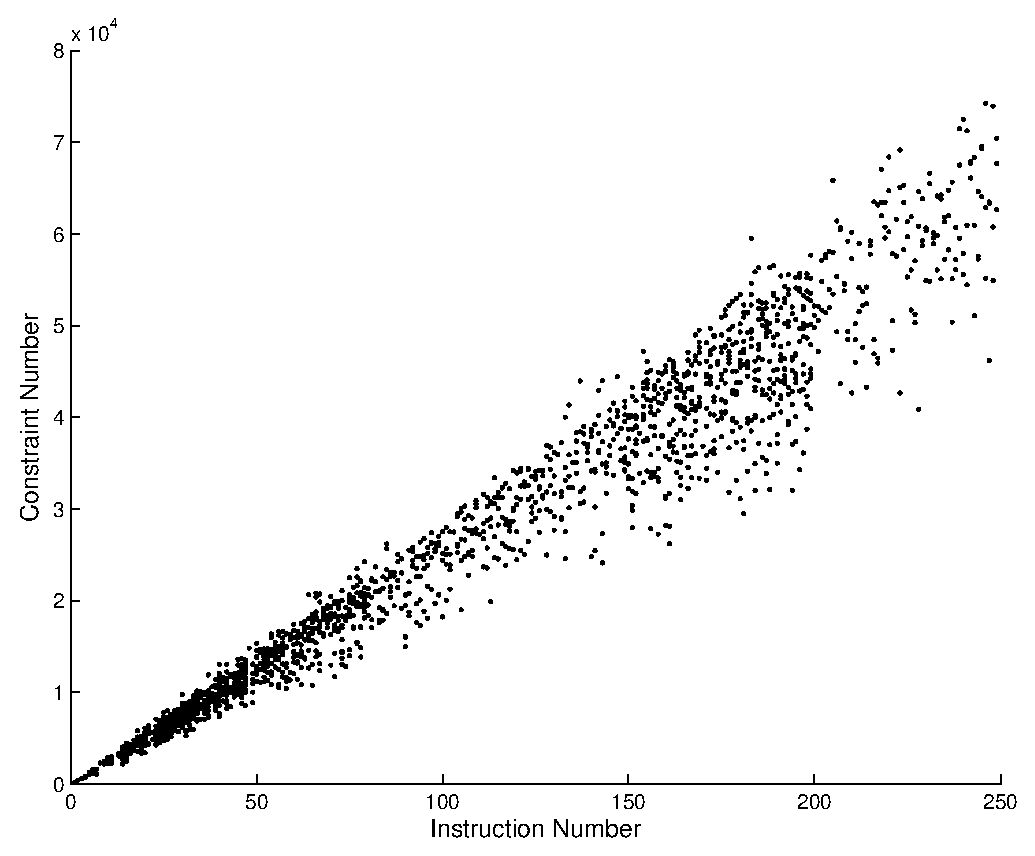
\includegraphics[width=4in]{figures/inst-cons.eps}
\caption{The number of constraints as a function of number
of IR instruction.}
\label{fexp.inst.con}
\end{figure}
\begin{figure}[htbp]
\centering
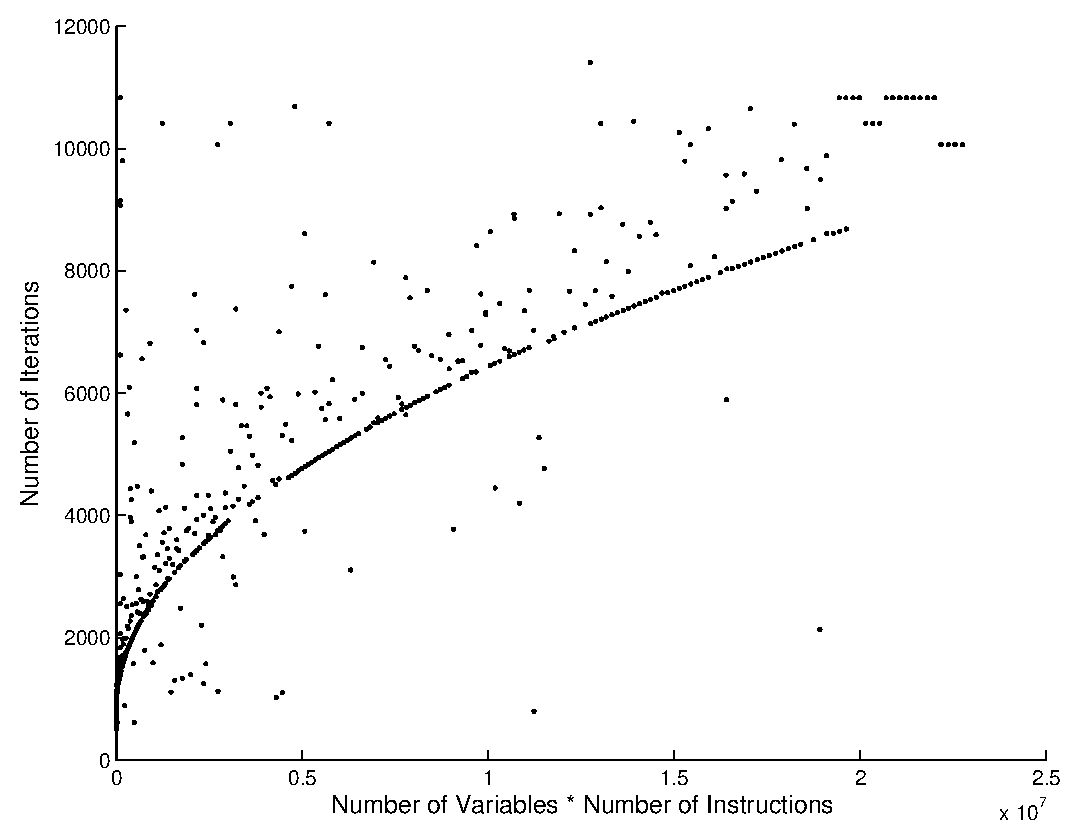
\includegraphics[width=4in]{figures/iter_linear.eps}
\caption[The number of iterations as a function of.]{The number of iterations as a function of
(the number of variables $\times$ the number of IR instructions).}
\label{fexp.iter.con}
\end{figure}

An interesting observation I found is that the preferred register tag
helps to improve the performance. Comparing to an ILP-based register
allocator which allocates register from scratch, the preferred
register tag is a hint to the solver and can reduce the number of
iterations that solver needs to try.  As an extreme case, I also
tested misleading preferred register tags, e.g., variables are
assigned to the preferred register tag randomly, I found the solver
may need 2 or 3 times more iterations to solve.

To see how fast the problem can be solved, I conducted timing
experiments on Intel Xeon 3.6GHz processor running Fedora Linux 2.4.21
kernel. The physical memory size is 2GB while in the experiments, the
largest observed memory usage is less than 256
MB. Figure~\ref{fexp.time.con} shows that the average time required to
solve one iteration increase about linearly with the problem
complexity.  It usually takes the solver less than 175 seconds to
allocate registers for a chunk of 250 IR instructions. As a
comparison, it takes GCC-RA less than one second to solve the same
problem. While UCC-RA is much slower than GCC-RA, it is not a
significant problem for WSNs due to the following reasons: (i) sensor
applications are small programs limited by the memory size of the
sensor node; (ii) UCC-RA is applied only to the identified {\em
changed} chunks instead of the complete functions or the whole
application; (iii) it is worthwhile to trade the compilation time at
the server side, where both energy and computation power are abundant,
for the energy savings on sensor nodes where resources are highly
constrained.
\begin{figure}[htbp]
\centering
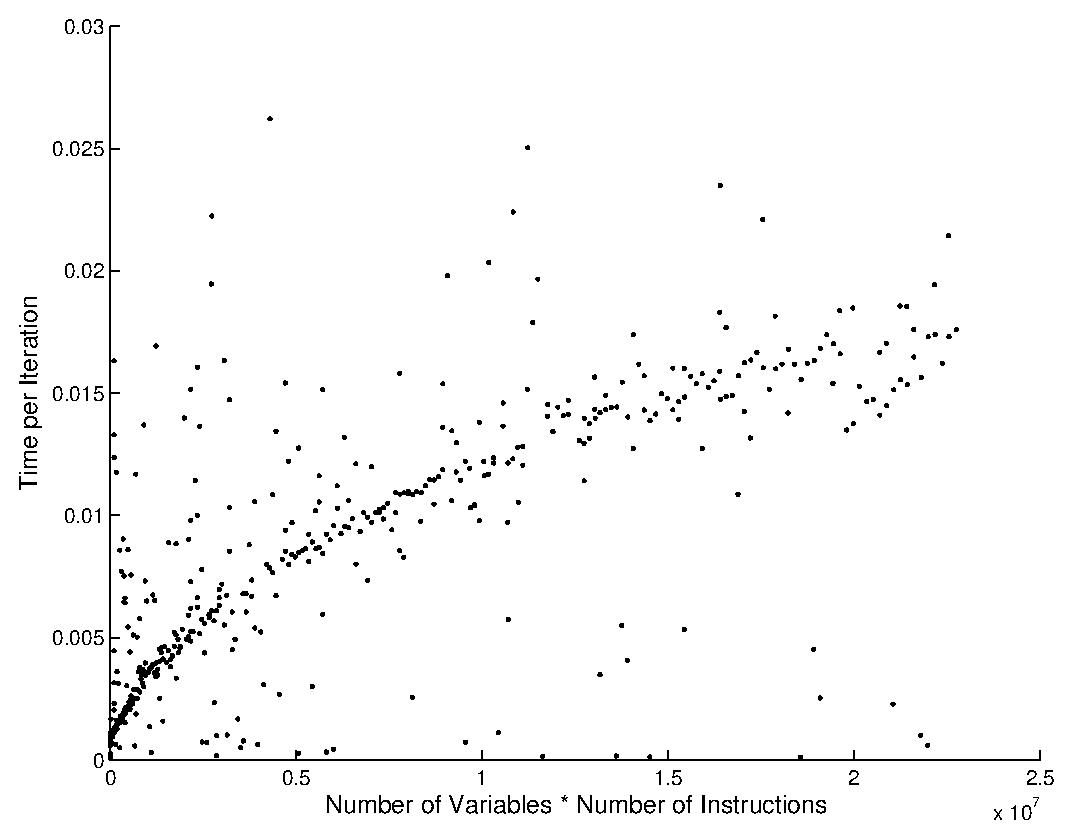
\includegraphics [width=4in]{figures/time_linear.eps}
\caption[The time to solve one iteration as a function of.]{The time to solve one iteration as a function of 
(the number of variables $\times$ the number of IR instructions).}
\label{fexp.time.con}
\end{figure}


I also performed experiments on testing whether approximating the
original non-linear integer programming problem with a linear problem
degraded the final results. I observed the same allocation decisions
for all the test cases with or without the approximation. The only
difference is that solving non-linear problems is orders of
magnitude slower than a linear problem.




\subsection{General purpose software update using UCC-DA}\label{exper-da}

In order to compare the performance of the proposed update-conscious compilation data
allocation scheme (UCC-DA) with GCC-DA, I used the manual generated general purpose 
benchmarks (M-G-14 $\sim$ M-G-19) list in
Figure~\ref{fbench.chg1} to generate the binary images and further the patch scripts.

The tradeoff of UCC-DA is between the stack size and the generate script size.
Keeping more local variables in the same location as the previous version reduces
the update script size. However, it may increase the stack size because when variables
are removed, the memory holes will not be filled because we want to 
keep the data allocation similarity. Thus, in the experiments, I evaluated both the
generated script size and the worst case stack usage using different data allocation
algorithms.

\subsubsection{Settings}

I used {\tt ncc}, the NesC compiler
included in TinyOS release, and {\tt avr-gcc}, the GNU C compiler
(GCC) re-targeted for AMTEL AVR micro controllers to get the baseline binary.

The generated binary is compared with the older version to generate
the update script. I compared the generated script size between GCC-DA
and UCC-DA.The wasted space threshold $SpaceT$ is set to 5 Bytes for the experiments.


Then, I used {\tt tos-ramsize}~\cite{ramsize}, the tool included in TinyOS release, to
generate the worst case stack size of the binary generated using
different data allocation schemes.

I used the TinyOS applications as my benchmarks. The simple applications
such as Blink, CntToRfms and CntToLeds, do not use many local variables,
because there is very little computation involved.
Thus, I chose the Advanced Encryption Standard (AES) application~\cite{aes} as the benchmark. 
It takes several steps to encrypt or decrypt the given data and in each step it does
some relatively complicated computation to get a temporary result and feeds that
to the next step. For example, in the  {\tt ShiftRow} step, it  
cyclically shifts the bytes in each row by a certain offset. 
Local variables are heavily involved here to store the temporary results.

The update benchmarks are created based on the AES application, 
shown in Figure~{fbench.chg1} M-G-14 $\sim$ M-G-19.
The medium size update includes code update that add or remove multiple
local variables in a single function. The large size update includes code update
that add or remove multiple local variables in multiple functions.


\subsubsection{The generated script size}

I first used UCC-DA and GCC-DA to generate the new binary, compared the
new binary with old one to generate the update script.
The script size comparison is shown in Figure~ref{da-upd}.
I set the wasted space threshold $SpaceT$ to be 5 Bytes for the experiments.

\begin{figure}[htbp]
\centering
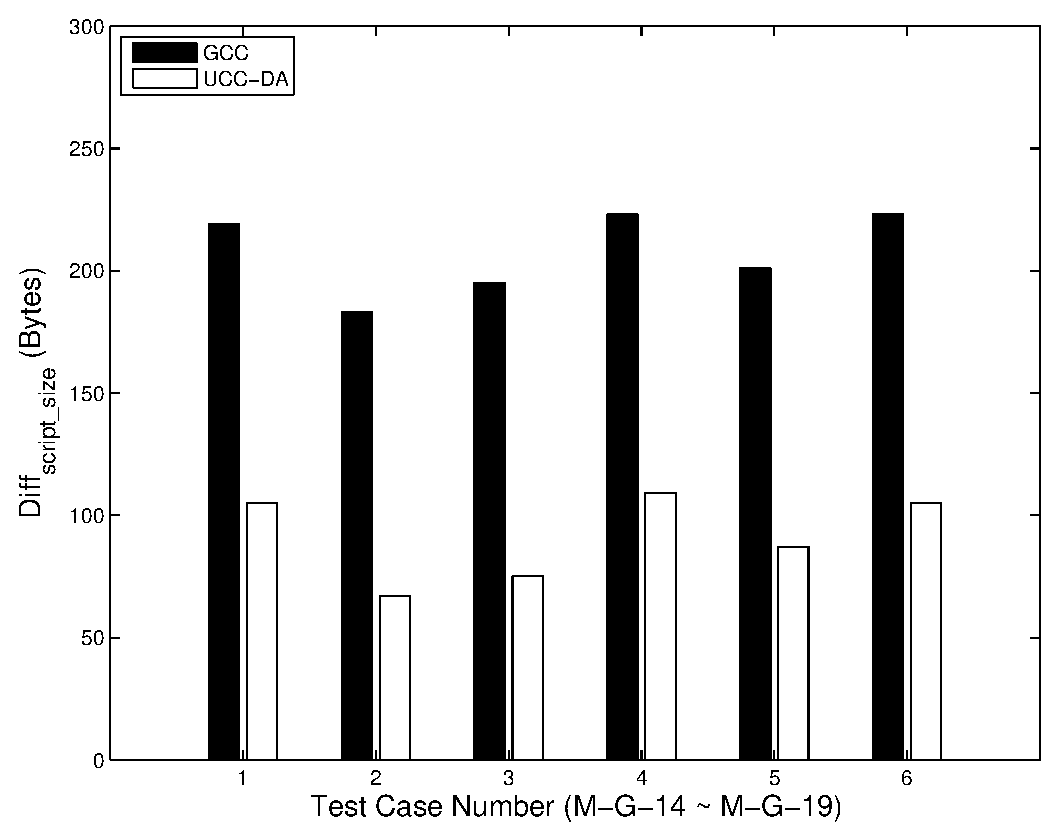
\includegraphics[scale=0.6]{./figures/da-upd.eps}
\caption{Script size comparison between UCC-DA and GCC-DA.}
\label{da-upd}
\vspace{-0.1in}
\end{figure}

Using UCC-DA, the script size can be reduced by 56\% on average.
New variables are always allocated at the top of the stack no matter where they are
declared, so that the unchanged variables that are declared after these new variables
do not have to be reallocated.
For the deleted variables, the memory hole will be left unfilled, if the total wasted memory size
 is smaller than the threshold $Space_T$. Otherwise, the variable are selected
 to the fill up the holes based on the factor that is presented in ~\ref{factor}.
 Under the given threshold, the UCC-DA algorithm keeps most of the unchanged variables
in their original memory location, so that it minimizes the update to the memory access instructions
that access those variables.

\subsubsection{The wasted memory space}

The UCC-DA algorithm trades the memory space for the script size reduction. Keeping
the unchanged variables in place may cause memory holes if some variables are removed.
Thus, it may cause some memory waste and result in a larger worst-case stack size.
Figure~\ref{da-stack} compares the worst-case stack size of the binaries generated
by different data allocation algorithms.

\begin{figure}[htbp]
\centering
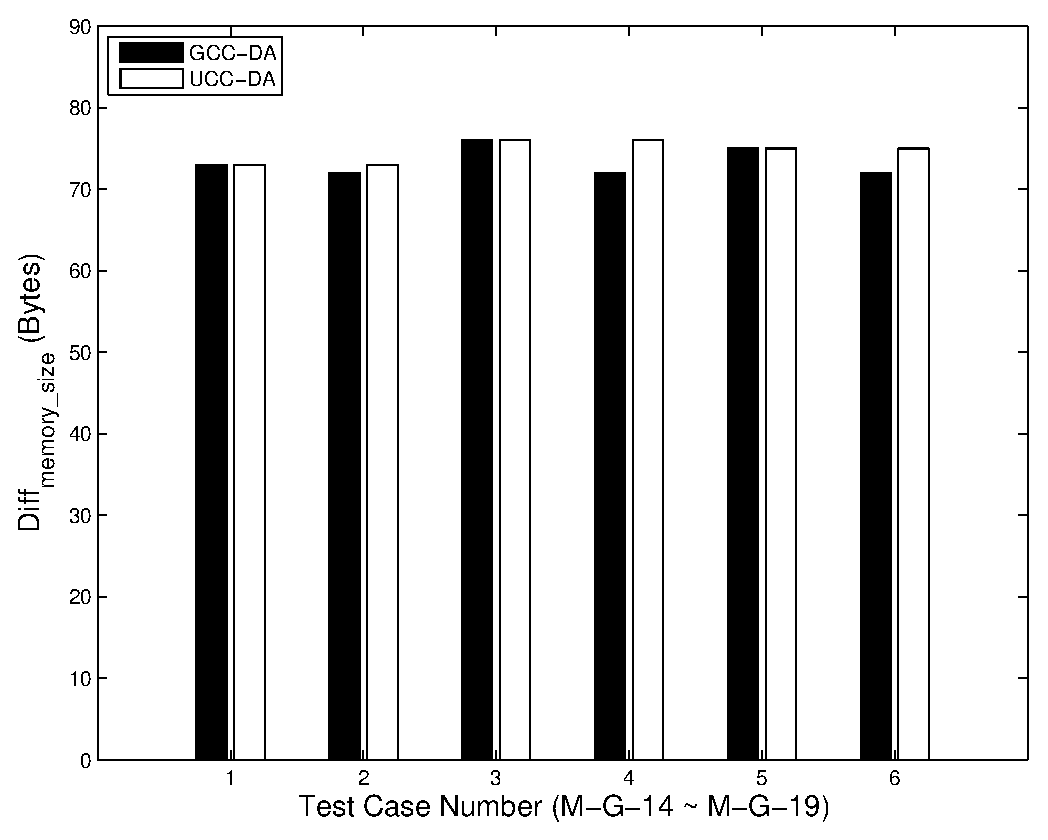
\includegraphics[scale=0.6]{./figures/stacksize.eps}
\caption{Worst-case stack size comparison between UCC-DA and GCC-DA.}
\label{da-stack}
\vspace{-0.1in}
\end{figure}

From the experiment results, using UCC-DA only increases the memory usage by 1.9\% on average,
yet reduces the script size by 56\%.
This is because only when the memory space taken by the removed variables is larger than
the memory space needed by the inserted variables, the memory space may be wasted.
In real life, the most common reasons of code updates are adding new features or fixing existing bugs.
Changing existing code and adding new code are more likely to happen instead of removing 
existing code.

\subsubsection{Tradeoff between wasted space and binary differences }

Shown in Figure~\ref{da-upd}, having the wasted space threshold $SpaceT$ set to be 5 Bytes gives 56\% script 
size deduction. Reducing this threshold may increase the script size, because more variables will
need to be moved to fill up the memory holes in order to meet this restriction.

Figure~\ref{da-tradeoff} shows such tradeoff.  I counted the number of instructions that need
to be updated due to data reallocation using GCC-DA.
Then, I compared that with the number of instructions that need to be updated due
to data allocation using UCC-DA, to compute the saved update \%.
With high wasted spaces threshold, the saved update \% is higher. 
Vice versa.

\begin{figure}[htbp]
\centering
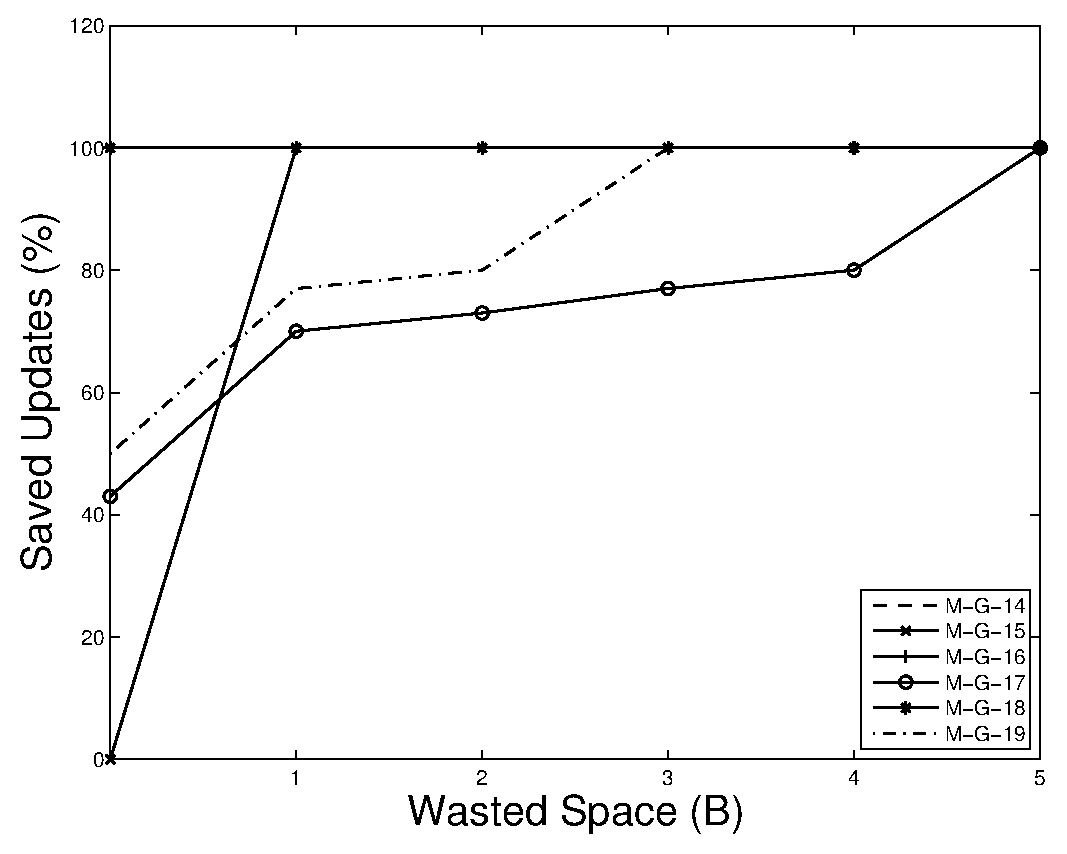
\includegraphics[scale=0.6]{./figures/spacetradeoff.eps}
\caption{Tradeoff between the worst-case stack size and the instruction updates.}
\label{da-tradeoff}
\vspace{-0.1in}
\end{figure}

From figure~\ref{da-tradeoff}, we can also see that the wasted space does not have to be high to
tolerant the instruction updates caused by data reallocation.
The worst-case stack size of the AES application is 67 Bytes. A 5 Byte memory waste
is large enough to tolerant all instruction updates caused by data reallocation, in the given
test cases.

An interesting observation is that even setting the threshold $SpaceT$ to be 0 Bytes can 
give some improvement, compared to the GCC-DA scheme. 
For example, test case M-G-14, M-G-16, and M-G-18 achieve 100\% update deduction
even when the threshold is set to 0 Byte.
This is happens when the memory space occupied by the deleted variables is smaller
than the space occupied by the inserted variables. 
Without the update-conscious scheme, the variables are ordered by the declaration 
sequence on stack. This may cause address shift to those unchanged variables
that are declared after these new variables. However, using the update-conscious scheme,
the new variables are first used to fill up the memory holes, and the extra new variables always 
allocated on top to the unchanged ones. Thus, these
unchanged variables will not be reallocated, so that less instruction updates will be
caused.

\subsection{General purpose software update using the integrated scheme}

\subsubsection{Performance evaluation using man-benches}
The experimental results in ~\ref{exper-ra} and ~\ref{exper-da} show that
using the Update-conscious register allocation and data allocation individually
can reduce the update script sizes by 71\% and 56\% representatively.
However, the performance loss caused by the update-conscious compilation schemes 
is very small, i.e., increasing the number of instructions in each execution by 
4.7\% and RAM usage by 1.8\%.

Integrating both the UCC-RA and UCC-DA schemes should combine the benefits
caused by both algorithms and reduce the script size even more.
I implemented the integration algorithm proposed in ~\ref{integration} and
ran the integration algorithm on the manual cases M-G-14 $\sim$ M-G-19.
The maximum wasted space threshold is set to be 5 bytes. The generated 
script size comparison is shown in Figure~\ref{general-inte}.

\begin{figure}[htbp]
\centering
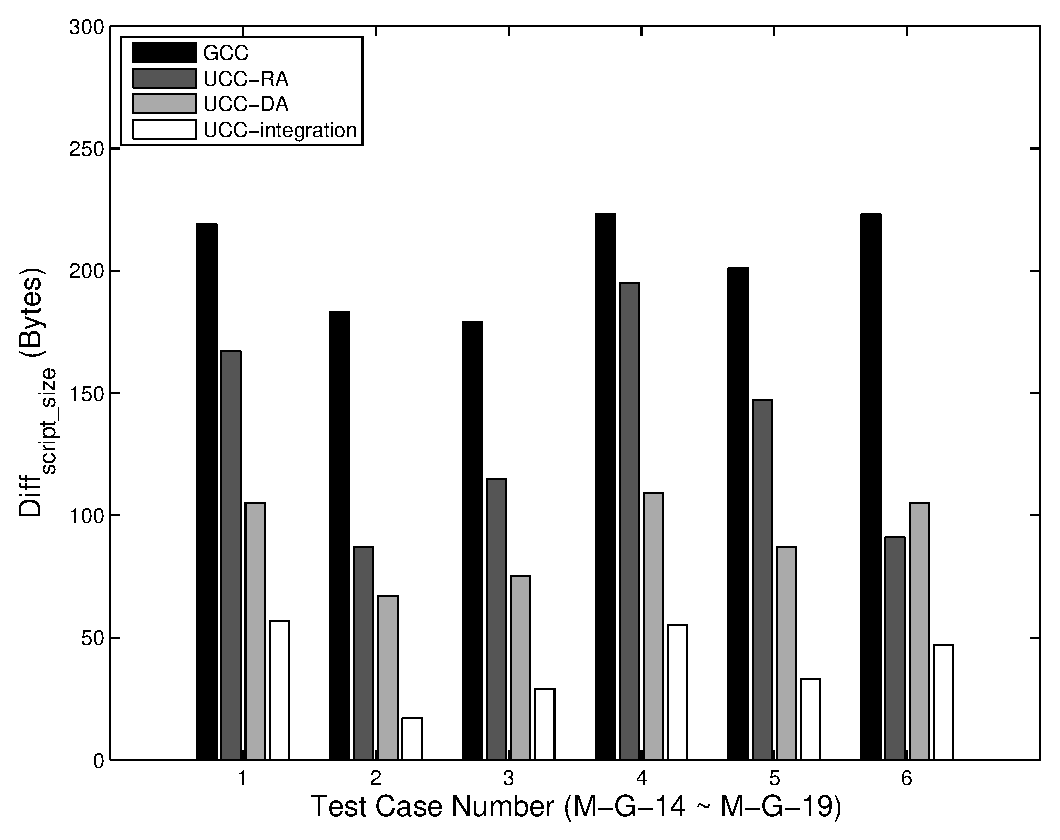
\includegraphics[scale=0.6]{./figures/inte-upd.eps}
\caption{Script size comparison between the integrated scheme and the baseline scheme.}
\label{general-inte}
\end{figure}

As shown in Figure~\ref{general-inte}, the integrated scheme produce the
smallest scripts compared to the individual UCC-RA and UCC-DA schemes. 

For these test cases, using the integrated scheme does not introduce any extra
run-time overhead. The reason is that the sensor applications are very simple that
the it has a low register pressure. For the presented test cases, the UCC-RA scheme can 
always find free registers to store the variables that are not tagged with a preferred
register. Thus, no extra move or spill instructions are introduced.


\subsubsection{Performance evaluation using real-benches}
I used the real general purpose benchmarks (R-G-1 $\sim$ R-G-6)
listed in Figure~\ref{fdeluge.src} to study the performance tradeoffs and
energy savings for real software update cases.
I used both GCC and UCC to get new binaries after each update, and then generate the update scripts according using update primitives described before. These scripts are distributed to the network using
the proposed MCP protocol and Deluge protocol to compare the network traffic and time savings.


Figure~\ref{fdeluge.data} shows the comparison results which include the number of script instructions per each type of primitive, and the final script size (bytes) for these two compilation techniques. In the case study, I did not add new instructions such that the performance is the same.

\begin{figure}[htbp]
\begin{center}
\begin{small}
\begin{tabular}{||p{0.5in}||p{0.38in}|p{0.15in} p{0.15in} p{0.2in} p{0.2in} p{0.15in}||
                           p{0.38in}|p{0.15in} p{0.15in} p{0.2in} p{0.2in} p{0.15in}||} \hline

Case \# & GCC Script Size (bytes) & \#A & \#R & \#P & \#C & \#L &  
          UCC Script Size (bytes) & \#A & \#R & \#P & \#C & \#L  \\ \hline \hline

R-G-1 &  \bf249 & 4&3&22&30&0    &\bf5  & 1&0&0&2&0  \\  \hline
R-G-2 &  \bf557 & 6&3&52&62&0    &\bf191& 8&3&1&4&0  \\  \hline
R-G-3 &  \bf447 & 2&1&39&43&0    &\bf12 &3&3&0&4&0   \\  \hline
R-G-4 &  \bf605 & 1&1& 4& 7&0    &\bf512 &6&0&1&8&0  \\  \hline
R-G-5 &  \bf277 & 0&4&31&36&0    &\bf35 &3&1&0&3&0  \\  \hline
R-G-6 &  \bf3981& 12&6&143&162&0 &\bf1069 &2&2&1&6&2 \\  \hline

\end{tabular}
\end{small}
\end{center}
\caption[Script size comparison for real purpose updates.]{Script size comparison for real general purpose updates (\#A: add primitive; \#R: remove primitive; \#P: replace primitive; \#C: copy primitive; \#L: clone primitive).}
\label{fdeluge.data}
\end{figure}

The average script size deduction for all the 6 test cases is 55\% comparing with GCC. This is because UCC reduces the instructions that need to be updated, thus the number of update primitives in the script is reduced. In addition, I found that when more instructions need to be updated, the code tends to be divided into smaller pieces, which results in more {\tt copy} primitives. For example in case R-G-3, UCC reduces the number of {\tt replace} primitives from 39 to 0, and {\tt copy} primitives from 43 to 4, which results in a 97\% script size deduction.

Notice that the {\tt clone} primitive is not frequently used in the script. This is because when the number of the instructions that can be ``cloned'' from the original code is not big enough, using {\tt replace} primitive is more efficient. For example, if there are {\tt N} instructions that can be ``cloned'' from the original code, which means that they are the same with the related instructions in the original code except for the register assignments, and a one-one mapping can be created between the register assignments in the two versions. The number of such register assignment mappings is {\tt M}. 
In such situation, I can use both {\tt clone} primitive and {\tt replace} primitive to represent the code updates. And the overhead of using each primitive is shown in the following equations.

\begin{small}
\begin{eqnarray}
Cost_{clone} = 5 + 2*M\\
Cost_{replace} = 1 + 2*N\\
Cost_{clone} < Cost_{replace} \Rightarrow N-M > 2
\label{clonevsreplace}
\end{eqnarray}
\end{small}

As shown in Equation \ref{clonevsreplace}, only when $N-M > 2$ is satisfied, I can gain more benefit by choosing the {\tt clone} primitive.

\subsection{DSP software update pre-dissemination}

In order to compare the performance of the proposed update-conscious compilation data
allocation scheme (GCC-DA) for DSP applications and the CSOA/CGOA schemes, I used the manual generated DSP
benchmarks (M-D-1 $\sim$ M-D-5)
list in Figure~\ref{dsp-bench} and Figure~\ref{dsp-manual} to generate the binary image
and further the patch script using the proposed script primitives.
Then, I used the automatically generated DSP benchmarks to study the performance tradeoffs
for more general cases.

\subsubsection{Settings}
I have implemented the proposed update-conscious ICSOA/ICGOA algorithms. I chose the Lance Compiler\cite{lance} to convert the source code (C code) into intermediate representations (IRs) from which the access sequence and interference graph are extracted. I selected the DSPstone\cite{dspstone} benchmark suite that is widely used to measure the performance of DSP compilers. I adopted CSOA-Offsetstone\cite{offsetstone} as the baseline CSOA and implemented ICSOA on top of it. 
%
%I evaluated the impact as the number of variable interferences that are added by the code update, and whether these new interferences conflict with existing variable partitioning result. An interference conflict happens when two coalesced variables (in the old assignment) have overlapped live ranges and thus cannot be coalesced anymore.


\subsubsection{Performance evaluation using man-benches}
\textbf{Single offset assignment}
Figure \ref{update} compares the software update overhead for CSOA and ICSOA. I used three script formats to do the comparison.
\begin{itemize}
\itemsep 0pt
\item
{\it Simple code update script} that uses only the simple functional primitives;
\item
{\it Advanced code update script} that uses all types of the functional primitives;
\item
{\it Context-aware update script} that uses both functional and data primitives.
\end{itemize}

Using the same script generator with ICSOA, the update script size can be reduced by 32\%.
This is because that the update-aware scheme follows the variable coalesces and offset assignment of the old code. The generated code has better code similarity to the old version in terms of both offset assignment and instruction addressing mode. In Test-Case M-D-1, the code update is very small such that the difference between the old and new offset assignments is not big. I did not see much benefit using ICSOA over CSOA. 

When comparing different script generators, I observed that  the advanced script generator produces a smaller script due to its usage of the {\it insert\_access} primitive. When there is no variable access insertion but contains removal or update in the code update, the two script generators produce the same script i.e. Test-Case M-D-4 and M-D-5.


The {\em context-aware} script generator produces smaller scripts when the code update is medium. Instead of sending individual instruction differences, it just sends out the data allocation differences, from which each node generates the new binary by itself i.e. Test-Case M-D-4 and M-D-5. I see a significant script size reduction by using this scheme. 
Adopting context-aware script tends to incur large complexity i.e. Test-Case M-D-1 and M-D-3 where I see a small script size increase due to the complexity to specify the offset assignment change. 


\begin{figure}[htbp]
\centering
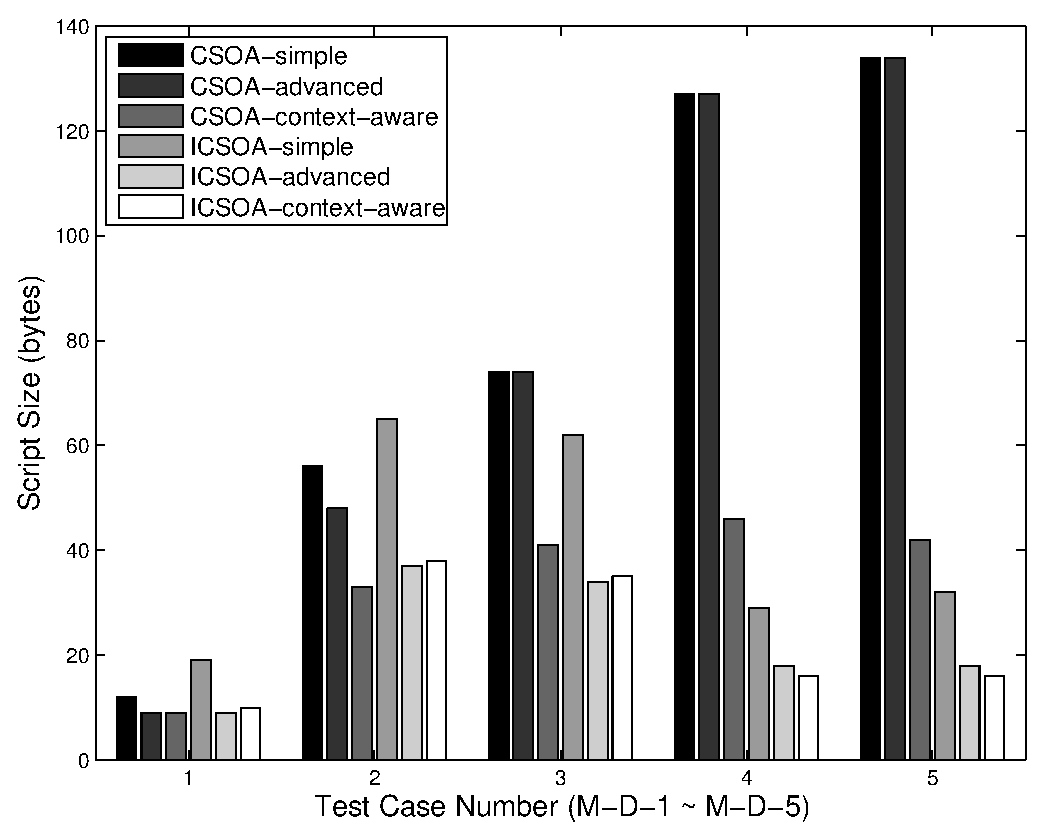
\includegraphics[scale=0.6]{./figures/update1.eps}
\caption{Script size comparison between ICSOA and CSOA ($Num_{addr\_reg} = 1$).}
\label{update}
\vspace{-0.1in}
\end{figure}

\textbf{General offset assignment}
When there are multiple ARs, Figure \ref{update2} compares CGOA and ICGOA schemes with the different script generators. 

\begin{figure}[htbp]
\centering
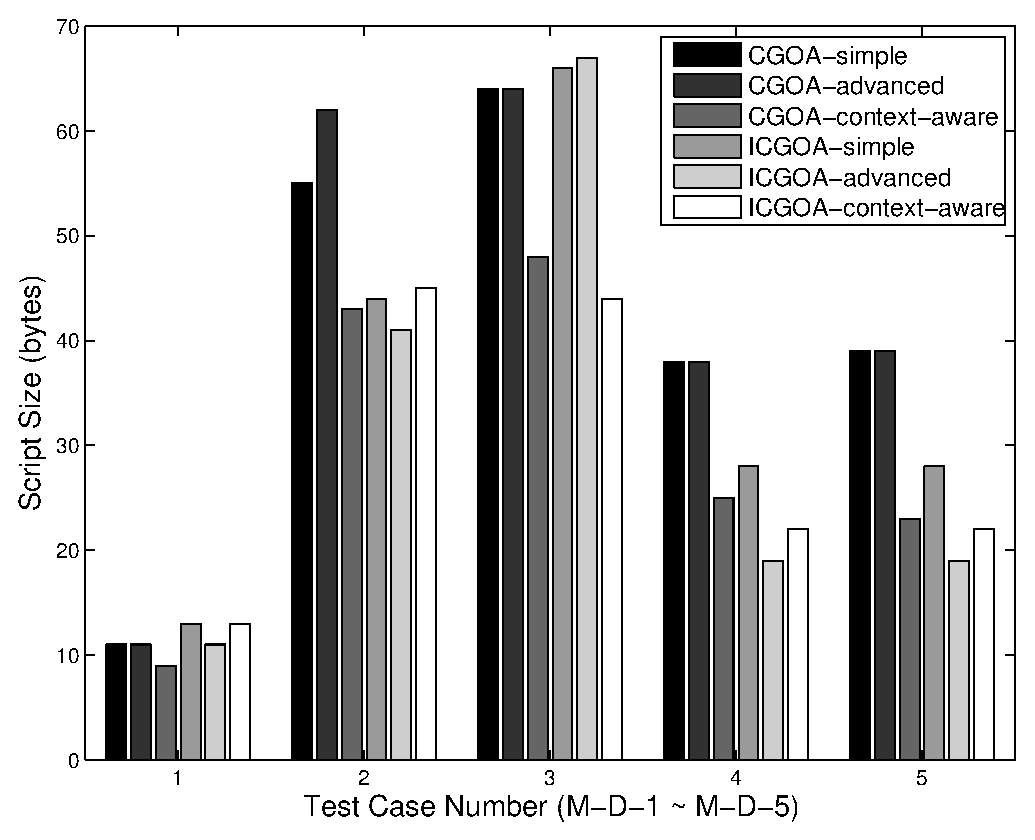
\includegraphics[scale=0.6]{./figures/updatem.eps}
\caption{Script size comparison ICGOA and CGOA($Num_{addr\_reg} = 2$).}
\label{update2}
\vspace{-0.2in}
\end{figure}

When there are more ARs, recompiling the program results in large changes in both the variable
partition and offset assignment. For Test-Case 3, CGOA with context-aware script has larger size than that with simple script. This is because that the significant variable partition change and requires more primitives to specify the new offset layout. 

In conclusion, ICSOA/ICGOA is preferred when there are medium changes while recompilation is preferred when the change is small or large.


In this paper I evaluated the static code quality i.e. the number of instructions in the new binary produced by CSOA and ICSOA schemes. An alternative approach is to evaluate the dynamic code quality i.e. the runtime instruction counts with given execution profiles. Although the latter provides more accurate evaluation, as I discussed in the introduction section, embedded mobile systems can periodically recharge the battery, so the execution overhead is less critical compared to its the communication overhead.

\textbf{Single offset assignment}
As shown in Figure \ref{exetotal}, ICSOA produces about the similar number of instructions as CSOA. On average, the binary generated by ICSOA is 10\% larger than the binary generated by CSOA. And for the worst test case, i.e. Test-Case 3, the binary generated by ICSOA is 23\% larger than CSOA. Because the ICSOA scheme incrementally does the data allocation based on the {\it coalesced access graph} of the old version, the old variable coalescing result is kept in the new version to improve code similarity. As a result, the code generated by ICSOA is not as efficient. 

\begin{figure}[htbp]
\begin{center}
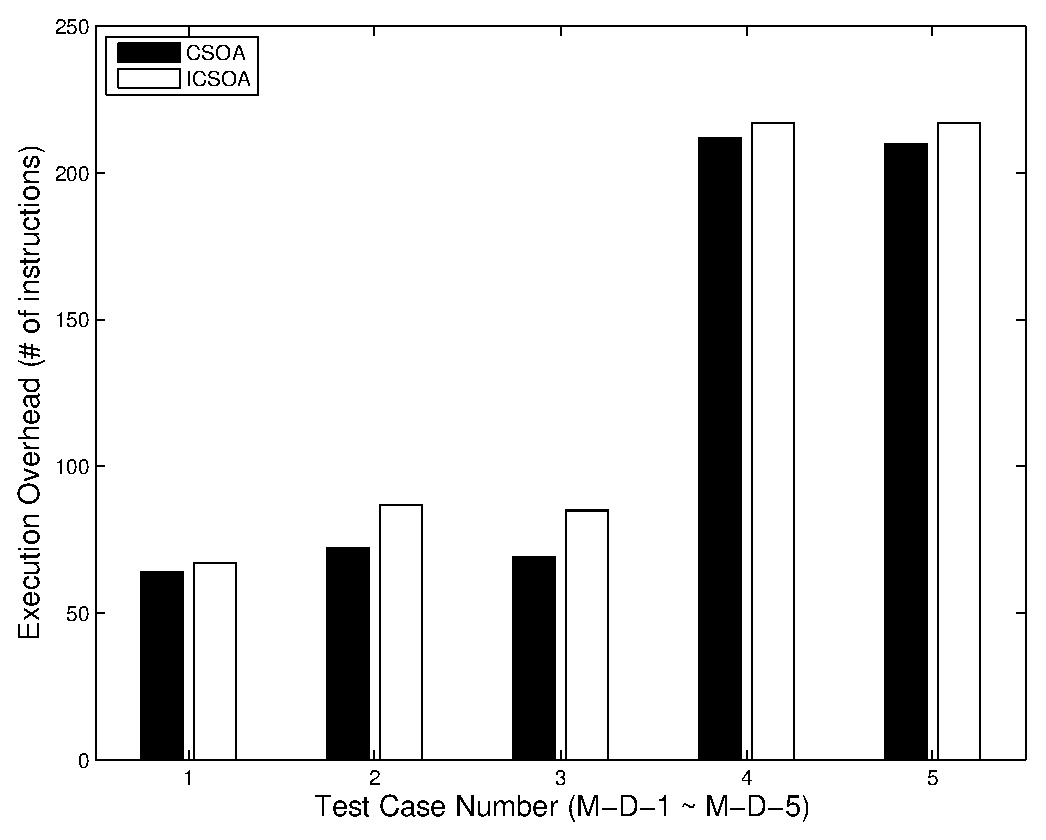
\includegraphics[width=4in]{./figures/da-exe1.eps}
\caption{Code quality comparison between CSOA and ICSOA.}
\label{exetotal}
\end{center}
\vspace{-0.2in}
\end{figure}


To better understand the code quality difference between two approaches, Figure \ref{exebreakdown} shows the breakdown of the execution overhead. I separated the new code at the intermediate representation (IR) level into the changed and unchanged parts. I then create their mapping to the binary level code segments.


\begin{figure}[htdp]
\begin{small}

\begin{center}
\begin{tabular}{|p{0.5in}|p{0.2in}p{0.2in}p{0.2in}p{0.2in}|p{0.2in}p{0.2in}p{0.2in}p{0.2in}|}
\hline 
Test &\multicolumn{4}{c|}{CSOA} & \multicolumn{4}{c|}{ICSOA} \\
Case\# & T1 & T2 & T3 & T4 & T1 & T2 & T3 & T4\\
\hline \hline
M-D-1	&0	&7	&1	&0	&0	&7	&2	&0	\\
								
M-D-2	&1	&7	&9	&0	&0	&8	&12	&3	\\
									
M-D-3	&1	&7	&7	&0	&0	&10	&12	&6	\\
									
M-D-4	&4	&24	&0	&0	&0	&24	&2	&1	\\
									
M-D-5	&4	&22	&0	&0	&0	&24	&2	&1	\\

\hline

\end{tabular}
\end{center}
\caption{Execution overhead breakdown.}
\label{exebreakdown}
\end{small}
\vspace{-0.1in}
\end{figure}


Due to the change to offset assignment, the same IR instructions may be different in the old and new code. The change could be categorized into two types: (1) updating the addressing mode of the related binary instructions, such as the first memory access in Figure \ref{recomdiff}; (2) adding addressing mode change instructions. The first type update does not change the instruction number as no extra instruction is added,
but for the second type, one extra instruction is added per change. 

To study the code quality, I divide the overhead into four categories as follows. T1-T3 shows how efficient the offset assignment algorithm is; and T4 shows how the extra patch affects the final result.
\begin{itemize}
%\itemsep 0pt
\item T1: AR loading instructions removed from the old code;
\item T2: AR loading instructions inserted into the old code;
\item T3: AR loading instructions inserted into the new code;
\item T4: ALU instructions inserted into the new code.
\end{itemize}

Comparing columns T1 and T2 of both CSOA and ICSOA in Figure \ref{exebreakdown}, I found that CSOA generates less binary instructions for the unchanged IR part. It removes more AR loading instructions, and inserts less such instructions. For the new code part, CSOA generates less AR loading instructions. When performing complete recompilation, CSOA uses the new access sequences and variable interferences of the whole function, and thus can generate the better offset assignment.

Column T4 shows the number of ALU instructions generated by compiling the new assembly code.  Since ICSOA needs to add patch variables to remove the interferences due to overlapped live ranges, it adds several ``move'' instructions in the code, which causes more T4 type instructions.

\textbf{General offset assignment} For the test case M-D-3 that has the largest code quality difference, I increased the number of available ARs, and found that with more available ARs, the code quality difference is reduced, as shown in Figure \ref{exe_ar}. The extra instruction number drops from 20\% to 6\% when the address register number is increased from 1 to 4. 
This is because with more ARs, the variables are partitioned into smaller sets. The software update tends to create less new interference and needs fewer patch variables. Fewer interferences result in less overhead in ICSOA. 

\begin{figure}[htbp]
\begin{center}
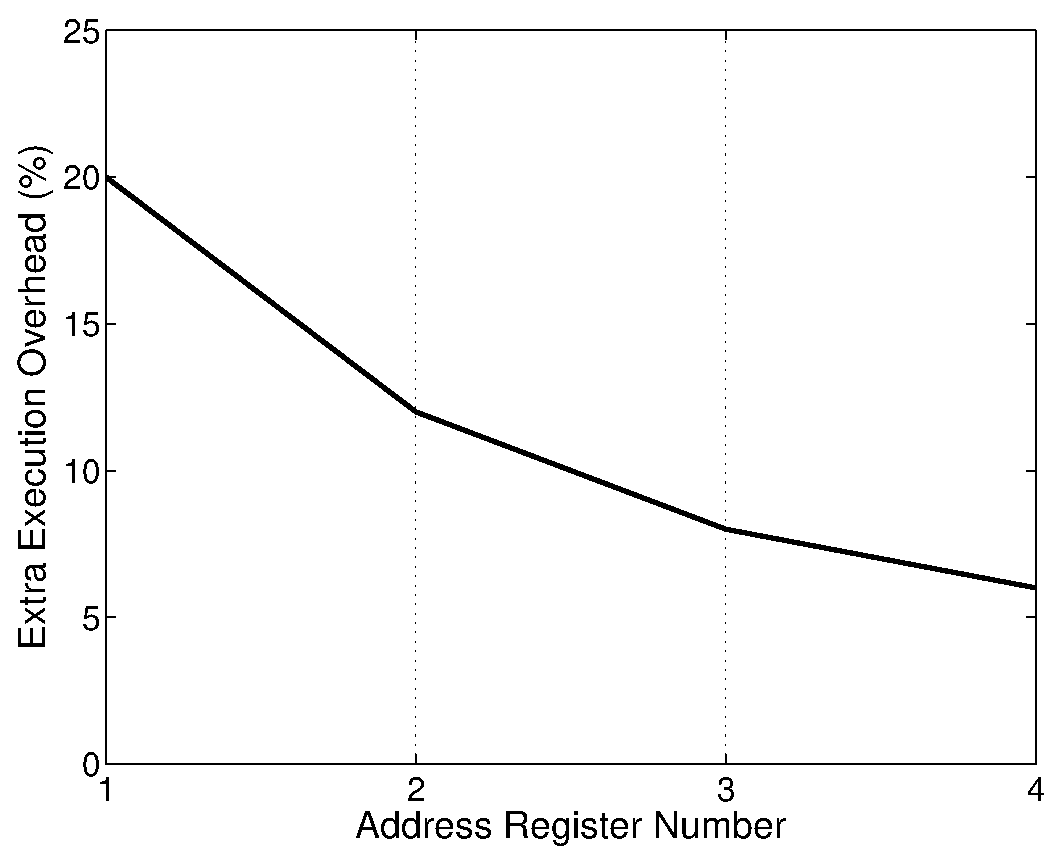
\includegraphics[width=4in]{./figures/exe_ar.eps}
\caption{Code quality comparison between ICGOA and CGOA.}
\label{exe_ar}
\end{center}
\vspace{-0.2in}
\end{figure}

\begin{figure}[htbp]
\begin{center}
\includegraphics[scale=0.4]{./figures/da-energy.eps}
\caption{The energy savings for DSP applications.}
\label{energy-dsp}
\end{center}
\end{figure}

The update-conscious data allocation scheme trades the run-time code performance for the transmission overhead during software update. Thus, the overall energy savings depend on the number of the times that the target binary will execute before retiring. Figure~\ref{energy-dsp} shows the energy savings of ICSOA over CSOA as a function of 
$Cnt$, which is projected from the execution profiles and the code update frequency.



As we can see in Figure~\ref{energy-dsp}, with the increase of the execution number of one application, the overall energy savings that are achieved by using the update-conscious compilation scheme is reduced. This is because the energy saved in the one time binary transmission is overwhelmed by the extra run-time overhead. When a large $Cnt$ is predicted, the update-conscious compilation will fall back to the CSOA scheme in order to achieve overall energy efficiency. 

\subsubsection{Performance evaluation using auto-benches}
I next inserted changes randomly into a file ({\em verify.c}) to study the robustness of my proposed scheme. The inserted code involves the use of both existing and new variables. The ratio of these two types is 1:1, and the sizes of the inserted/changed code range from 5\% to 60\% of the original code. Given an update percentage, I randomly generated 500 test cases and reported the average.

The script size comparison is shown in Figure \ref{upd_rand_bar}. For all three types of the script generation schemes, incremental compilation scheme reduces more of the
update script size and thus the software update transmission overhead. However, the results show that I achieved the maximum script size reduction when the update percentage is between 10\% and 40\%. This is because ICSOA benefits more when most of the update is caused by the data allocation changes rather than new/updated instruction operations. When the update percentage is too big, i.e. larger than 40\%, most changes are new or updated instructions. When the update percentage is too small, i.e. smaller than 20\%, the data allocation table is less likely to change even with recompilation. Thus, the benefits from ICSOA are limited.


\begin{figure}[htbp]
\begin{center}
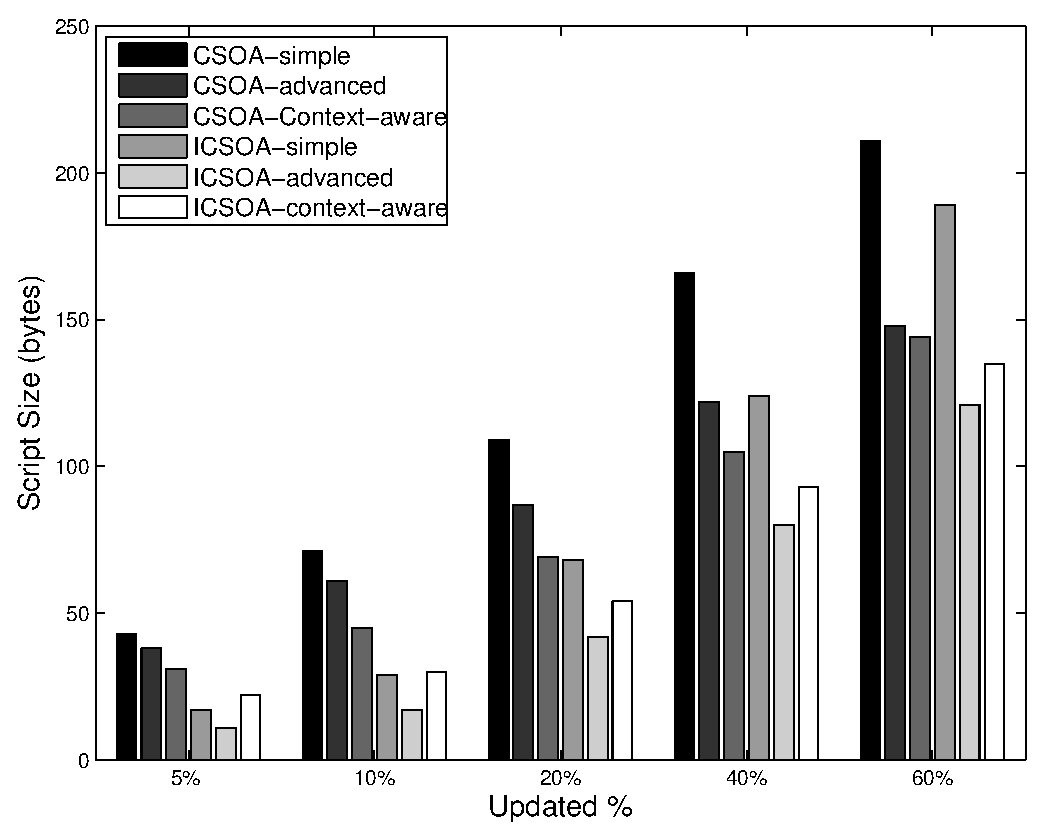
\includegraphics[width=4in]{./figures/upd_rand_bar.eps}
\caption{Script size comparison (scattered random new code insertion).}
\label{upd_rand_bar}
\end{center}
\vspace{-0.2in}
\end{figure}

The code quality is compared in Figure \ref{exe_rand_bar}. Larger code update percentage, i.e. over 40\%, has more live range extension of old variables, which produces more patch variables and instructions. Thus, the code produced by the recompilation scheme has a larger number of T4 type instructions; the code generated by the ICSOA scheme has a worse execution performance. 


\begin{figure}[htbp]
\begin{center}
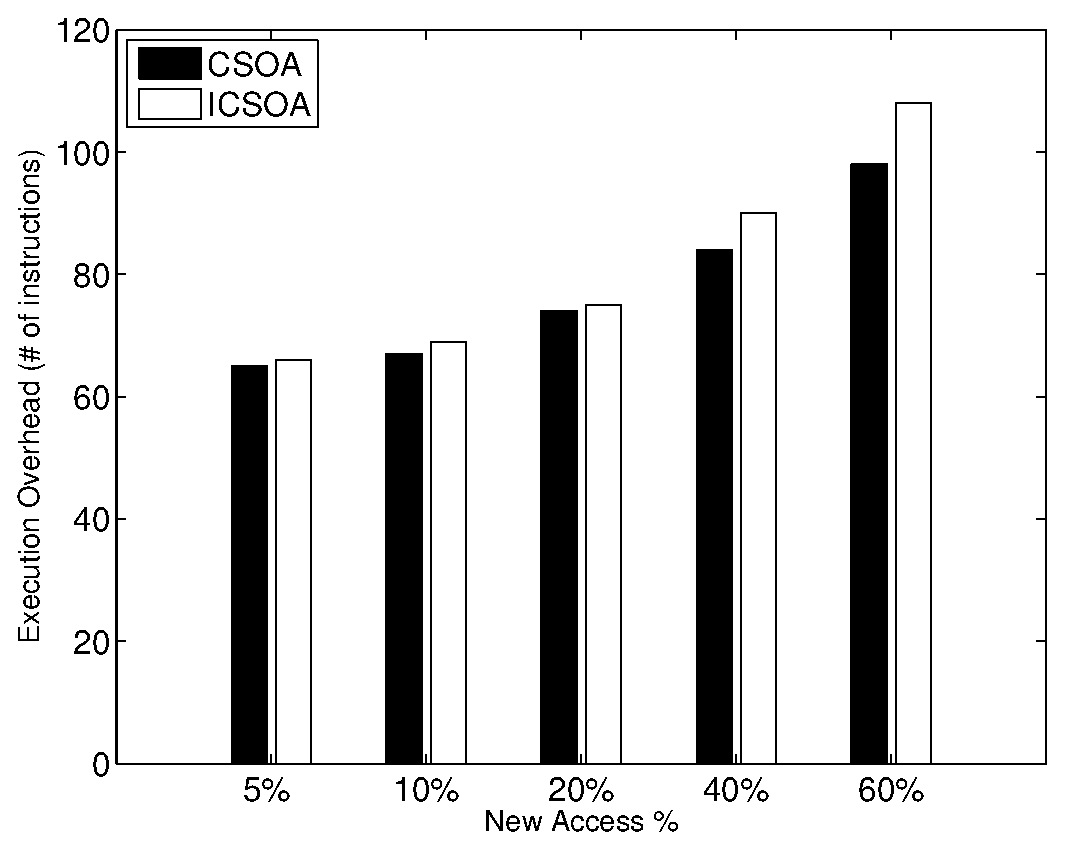
\includegraphics[width=4in]{./figures/exe_rand_bar.eps}
\caption{Code quality comparison (scattered random new code insertion).}
\label{exe_rand_bar}
\end{center}
\vspace{-0.2in}
\end{figure}


From Figure \ref{exe_rand_bar} and Figure \ref{upd_rand_bar}, I conclude that when the code update percentage is between 20\% and 40\%, using the update-conscious offset assignment scheme can save about 30\% of the transmission overhead, assuming that advanced script is used, with about 2\% extra instruction execution.


From the experimental results, I can also see that the simply using the code primitives works better with the incremental compilation scheme, and the context-aware primitives works better with the recompilation scheme.
This is because that the context-aware primitives trades updating individual instructions for setting up the auxiliary data structures and letting the sensors to construct these updates.
Thus, when I recompile the new version, a relatively great number of instructions are changed due to the data allocation differences, so the  context-aware primitives can gain more benefit by saving those updates. 
On the other hand, when I use the incremental compilation technique, the saving is not great enough to balance the spending in setting up the data structures, therefore, just using the code primitives is more beneficial. 


\subsubsection{Performance evaluation using real-benches}
I used the real general DSP benchmarks (R-D-1 $\sim$ R-D-3)
listed in Figure~\ref{dsp-bench} to study the performance tradeoffs and
energy savings for real software update cases.

Considering only the update-conscious data allocation scheme (UCC-DA) for DSP applications,
I compared the update script size, generated binary performance and long term energy savings
between the baseline CSOA scheme and the proposed ICSOA scheme.
With the consideration of both update-conscious data allocation (UCC-DA) and update-conscious
register allocation (UCC-RA), I did the comparison between the baseline CGOA scheme and ICGOA scheme.
The update scripts are then generated using different update primitives described before. These scripts are distributed to the network using the base Deluge protocol and the proposed MCP protocol to compare the network traffic and time consumption.

\begin{figure}[htbp]
\centering
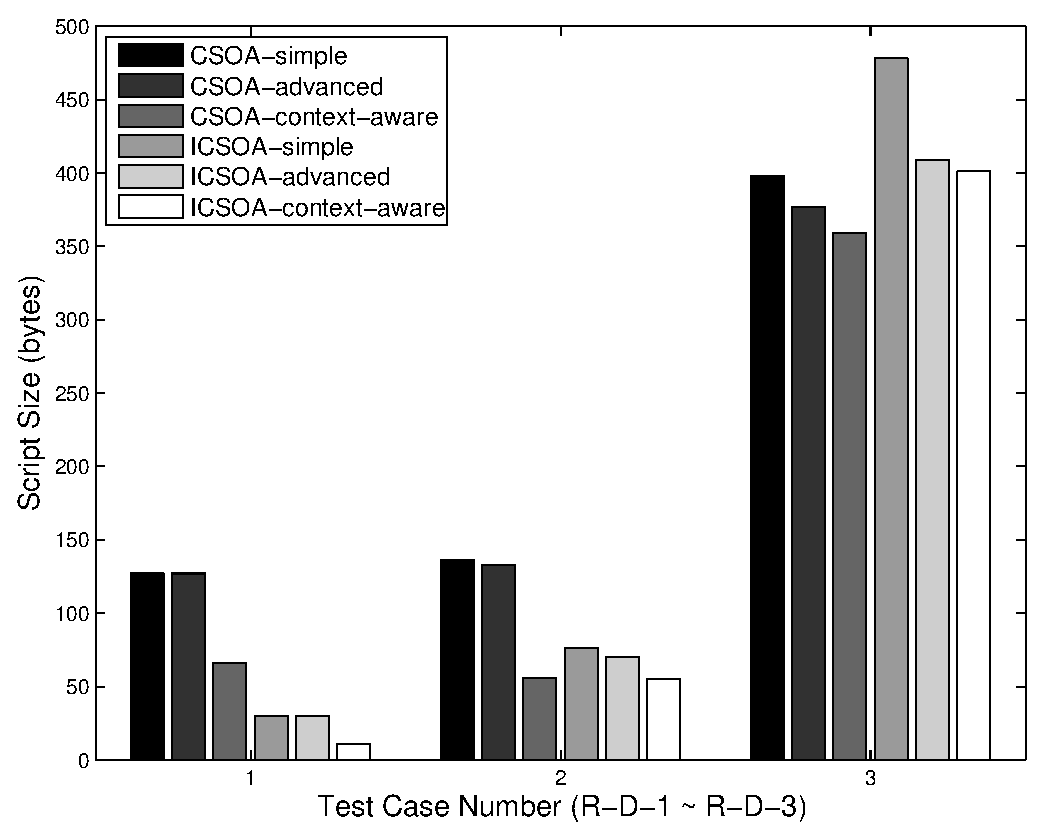
\includegraphics[scale=0.6]{./figures/update2.eps}
\caption{Script size comparison between CSOA and ICSOA ($Num_{addr\_reg} = 1$).}
\label{update-dsp-real}
\vspace{-0.1in}
\end{figure}

Figure~\ref{update-dsp-real} shows the generated script size comparison using different compilation techniques 
and update primitive sets. Here, test case R-D-1 and R-D-2 are medium level updates, while R-D-3 is a high level update. 

Comparison between \textbf{CSOA-simple} and \textbf{ICSOA-simple}, we can see that update-conscious data allocation (ICSOA) produces the binary that is more similar as the old binary when the update level is relatively low. When the code has significant changes, e.g. Test-Case R-D-3 introduces 32\% code changes, the old and new code segments are mixed, such that the benefit from keeping the old data offset assignment diminishes.

Comparison between \textbf{CSOA-simple} and \textbf{CSOA-advanced} shows the script size deduction that we can achieve using the advanced script primitives over the simple script primitives. The advanced primitives tend to take more effect when the code update level is higher. This is because they work under certain circumstances, e.g., only when the update involves inlined functions, the {\tt clone} primitive can help to reduce the script size, and higher level updates provide more opportunities for these primitives to take effect.

Comparison between \textbf{CSOA-simple} and \textbf{CSOA-data} shows the script size deduction that we can achieve using the   context-aware primitives over the simple script primitives. Although using the  context-aware primitives primitives increase the code regeneration overhead on the sensors, it helps to reduce the script size significantly, especially when the data allocation update is significant. For example, the baseline CSOA scheme compared to the ICSOA scheme produces a more different data allocation result from the old version.
The improvement achieved by the  context-aware primitives when using the CSOA compilation technique is higher than using the ICSOA compilation technique.

In real life, there are usually more than one address registers available on a DSP chip. The more the address registers that are available, the larger the solution space is. Without the knowledge of the old compilation results, regenerating the new binary may cause more data allocation differences. 

Figure~\ref{update2-dsp-real} shows the experimental results, for double address register situation.
Here, I compared the baseline CGOA scheme with the proposed ICGOA scheme. 

\begin{figure}[htbp]
\centering
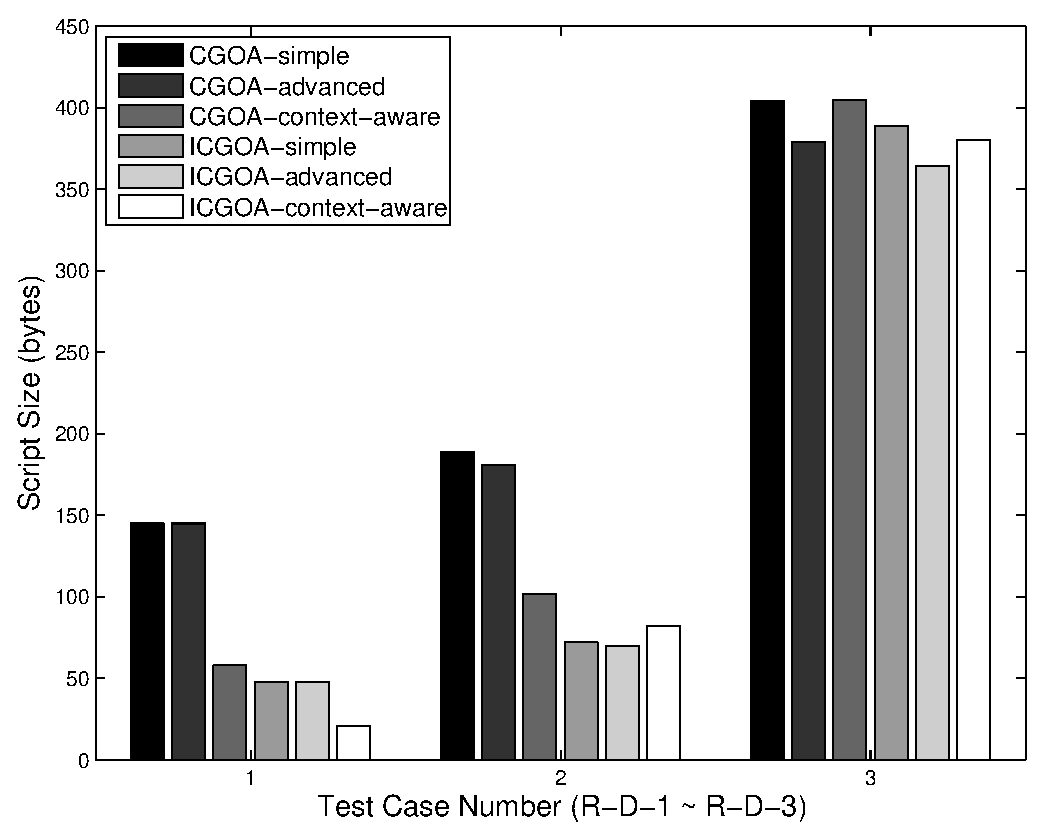
\includegraphics[scale=0.6]{./figures/updatem2.eps}
\caption{Script size comparison between CGOA and ICGOA ($Num_{addr\_reg} = 2$).}
\label{update2-dsp-real}
\vspace{-0.1in}
\end{figure}

We can see that when more address registers are available, the baseline scheme tends to generate the larger update scripts, which increases the improvement space of the update-conscious compilation techniques.

Figure~\ref{exe-dsp-real} shows the generated code performance comparison between the baseline CSOA scheme and the proposed ICSOA scheme. When code changes, inheriting the old data allocation result may not result in an efficient code. Thus, ICSOA generates more instructions compared to CSOA. For these real test cases, on average, ICSOA increases the run-time overhead by 3.7\%. 
\begin{figure}[htbp]
\centering
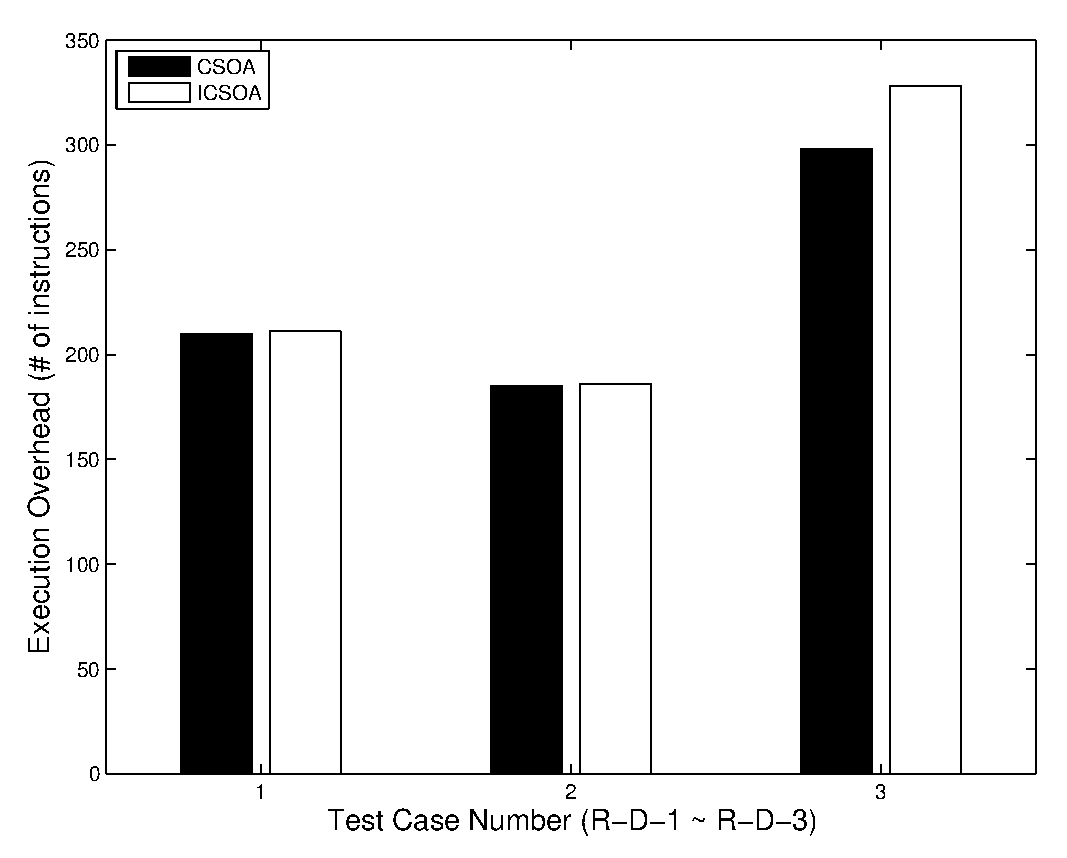
\includegraphics[scale=0.6]{figures/da-exe2.eps}
\caption{Code quality comparison between CSOA and ICSOA ($Num_{addr\_reg} = 1$).}
\label{exe-dsp-real}
\vspace{-0.2in}
\end{figure}


\section{Patch dissemination performance evaluation}
\subsection{Settings}
I implemented MCP on the TinyOS~\cite{tinyos} platform. For comparison, I also implemented Melete~\cite{melete} and studied various network settings using TOSSIM~\cite{tossim}. 

I simulated mesh MA-WSNs of different sizes. I set the default spacing factor to 15 and model the lossy communication channel using the tool provided by TinyOS. There are four applications each of which is uniformly distributed across the network. In the default setting, 30\% of the sensors have application {\tt A} and there is a request from the sink to reprogram 20\% of the other sensors to run {\tt A}. MCP disseminates the code from in-network sources instead of the sink. 

\subsection{Message overhead}

\begin{figure}[htbp]
\centering
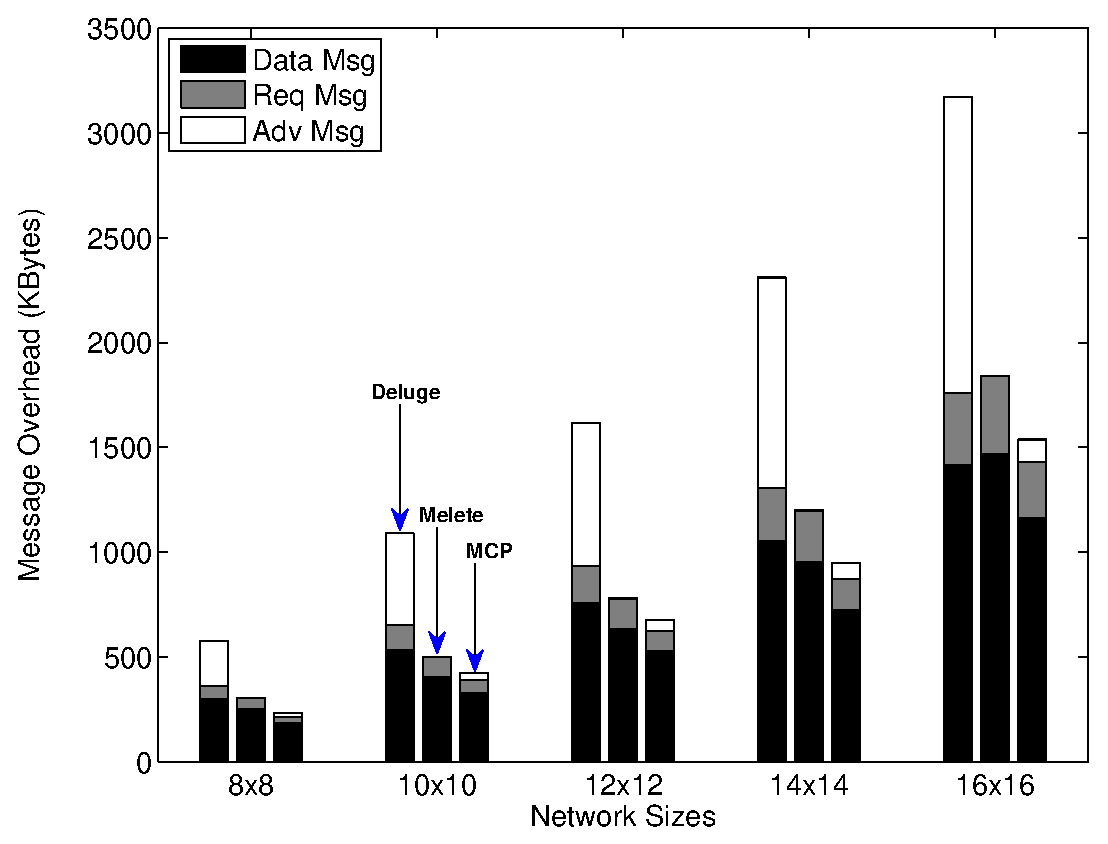
\includegraphics[width=4.2in]{figures/fsizes.eps}
\caption{Message overhead.}
\label{fmsg}
\end{figure}

Fig.~\ref{fmsg} shows the breakdown of the number of messages with different dissemination protocols. Without considering advertisement messages, Melete and Deluge have about the same message overhead, which was also reported in \cite{melete}. There are a large number of {\tt ADV} messages in Deluge, and a negligible number in Melete. The reason of such difference is Deluge depends heavily on incoming {\tt ADV} message, e.g., a sensor node only sends out new requests if it receives {\tt ADV} messages indicating its neighbors have more up-to-date data. Instead, in Melete, requesters receive the command from the sink code and then know the target application and its size. The requesters can proactively send out more requests after timeouts or receiving one complete page. The {\tt ADV} messages contribute to 37-40\% of the total message overhead in Deluge. 

My scheme takes a similar approach as Melete but requires some {\tt ADV} messages to update the AIT before, during and after the code switch. The {\tt ADV}'s overhead is low compared to the request and data transfer message overhead. On average my scheme reduces about 20\% of the message overhead from Melete. The main reason for this reduction is that Melete tends to have multiple responders within a small range and has a higher possibility of signal collision. MCP alleviates the problem by chosing one closeby source, which reduces the number of data packets in transmission.

\subsection{Completion time}

\begin{figure}[htbp]
\centering
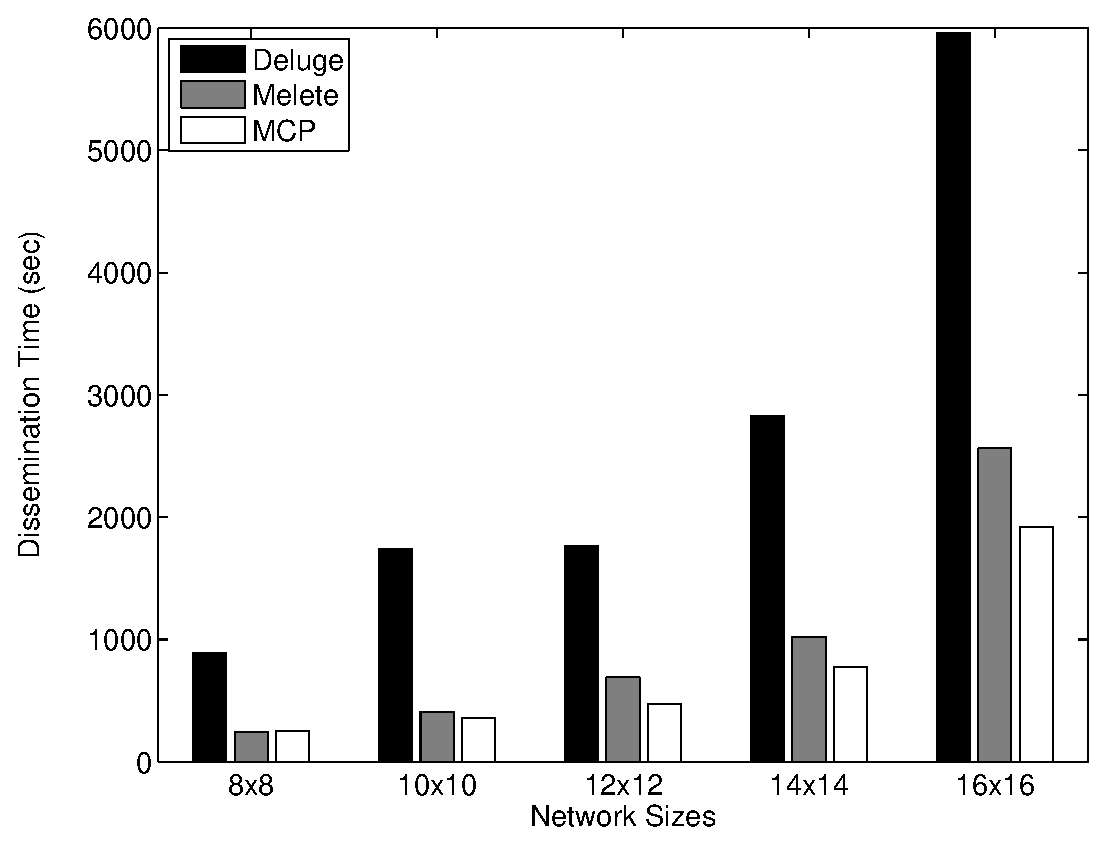
\includegraphics[width=4.2in]{figures/ftime.eps}
\caption{Dissemination time.}
\label{ftime}
\end{figure}

Fig.~\ref{ftime} compares the dissemination completion time of the different protocols. For the Deluge result, I record the time interval used by all requesters to complete the new code downloading. In practice, the Deluge protocol may still proceed to flood all sensors since it is not designed to update a subset of sensors. MCP requires less time to finish dissemination; on average it saves 45\% and 25\% over Deluge and Melete respectively.

\subsection{Sensitivity to node distribution}

\begin{figure}[htbp]
\centering
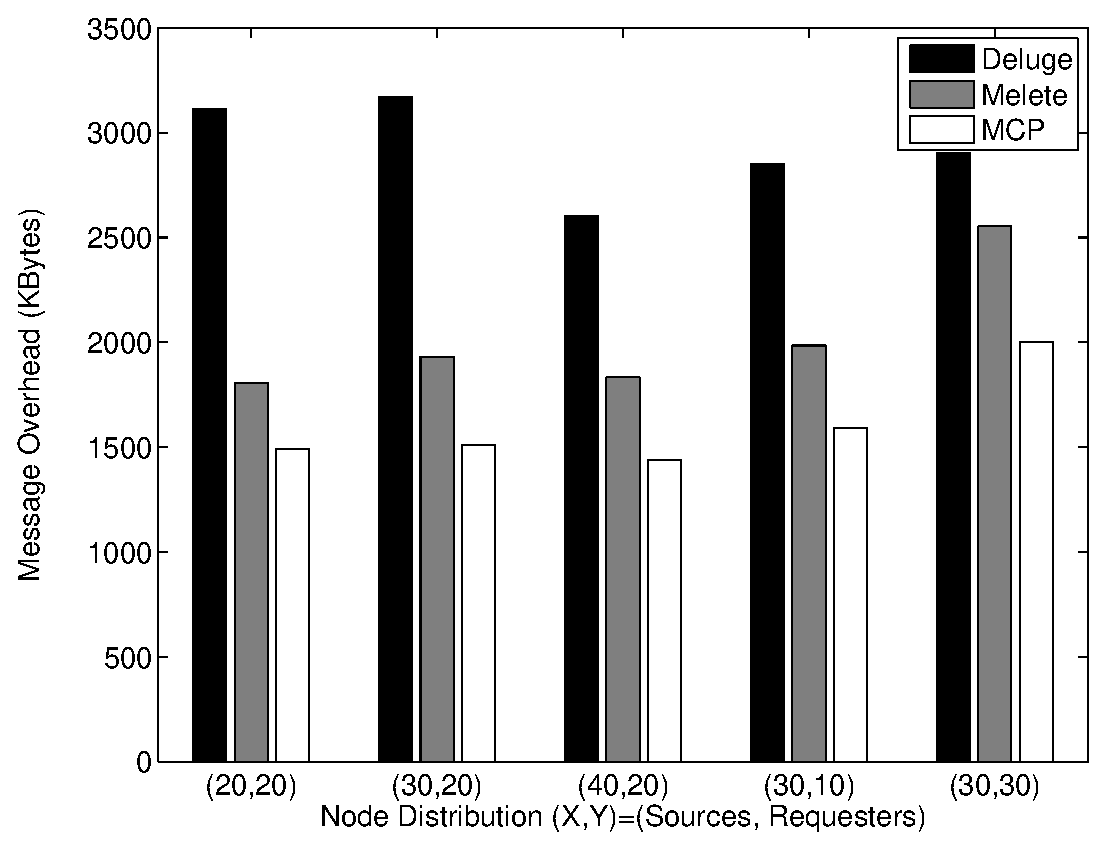
\includegraphics[width=4.2in]{figures/fdist1.eps}
\caption{Dissemination with different number of sources and requesters.}
\label{fsr}
\end{figure}

\begin{figure}[htbp]
\centering
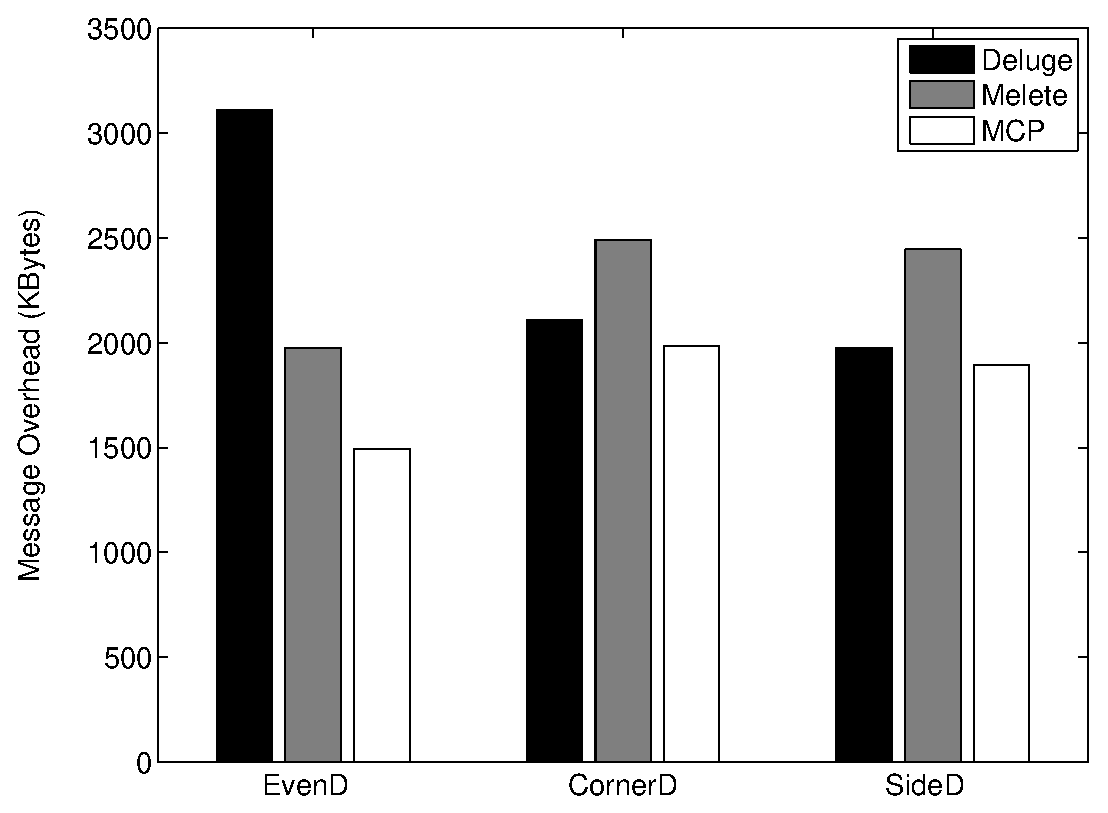
\includegraphics[width=4.2in]{figures/fdist3.eps}
\caption{Dissemination with uneven source/requester node distribution.}
\label{floc}
\end{figure}

Fig. \ref{fsr} illustrates message overhead with a different number of sources and requesters. I omit the dissemination time figure which exhibits similar results.
Along the X axis, (a,b) denotes that out of all the sensor nodes, a\% sources and b\% requesters are randomly selected in the field. I observed that the overhead tends to increase with more requesters and fewer sources. The difference is not significant.


Fig. \ref{floc} compares the message overhead when sources and requesters are distributed with location concentration. {\tt EvenD} denotes that all nodes are evenly distributed. {\tt CornerD} denotes that sources and requesters are distributed at the two diagonal corners of the rectangle field. {\tt SideD} denotes that sources and requesters are distributed along two sides of the field. From the figure, Melete has better performance than Deluge under even distribution. However, it generates significant conflicts and performs worse than Deluge when the nodes are unevenly deployed. MCP has consistently better results over Melete and Deluge. For the corner and side settings, MCP and Deluge are similar as almost all nodes are involved in the dissemination. 


\subsection{Sensitivity to application sizes}
Fig. \ref{fnumPage} shows message overhead with different application sizes. 
Due to the epidemic dissemination, Deluge exhibits approximately linear message overhead when
increasing the application size from 8 to 16 pages. Both Melete and MCP greatly reduce the communication overhead; however, they have slightly more than linear message overhead due to independent page requesting from requesters. MCP has a nearly constant message overhead reduction versus Melete, varying from 17.5\% for 8 pages to 18.1\% for 16 pages.

\begin{figure}[htbp]
\centering
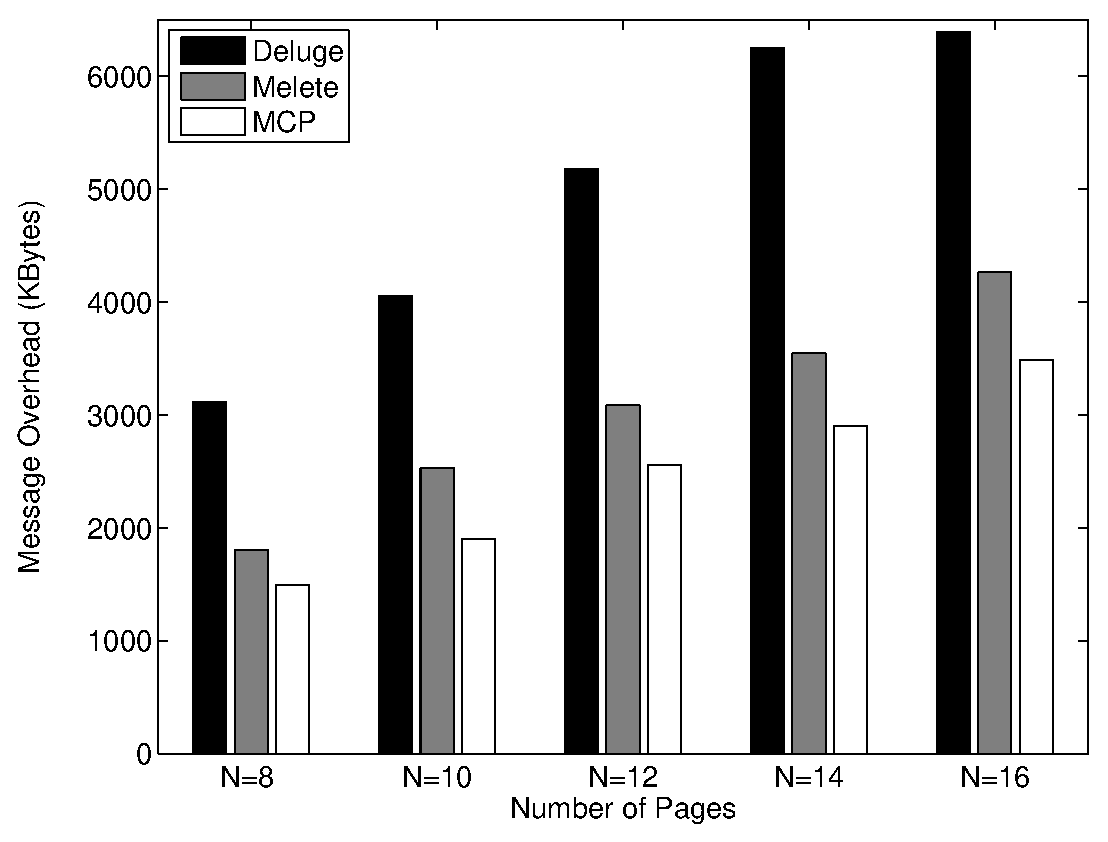
\includegraphics[width=4.2in]{figures/fdist2.eps}
\caption{Dissemination with different number of pages.}
\label{fnumPage}
\end{figure}
\begin{figure}[htbp]
\centering
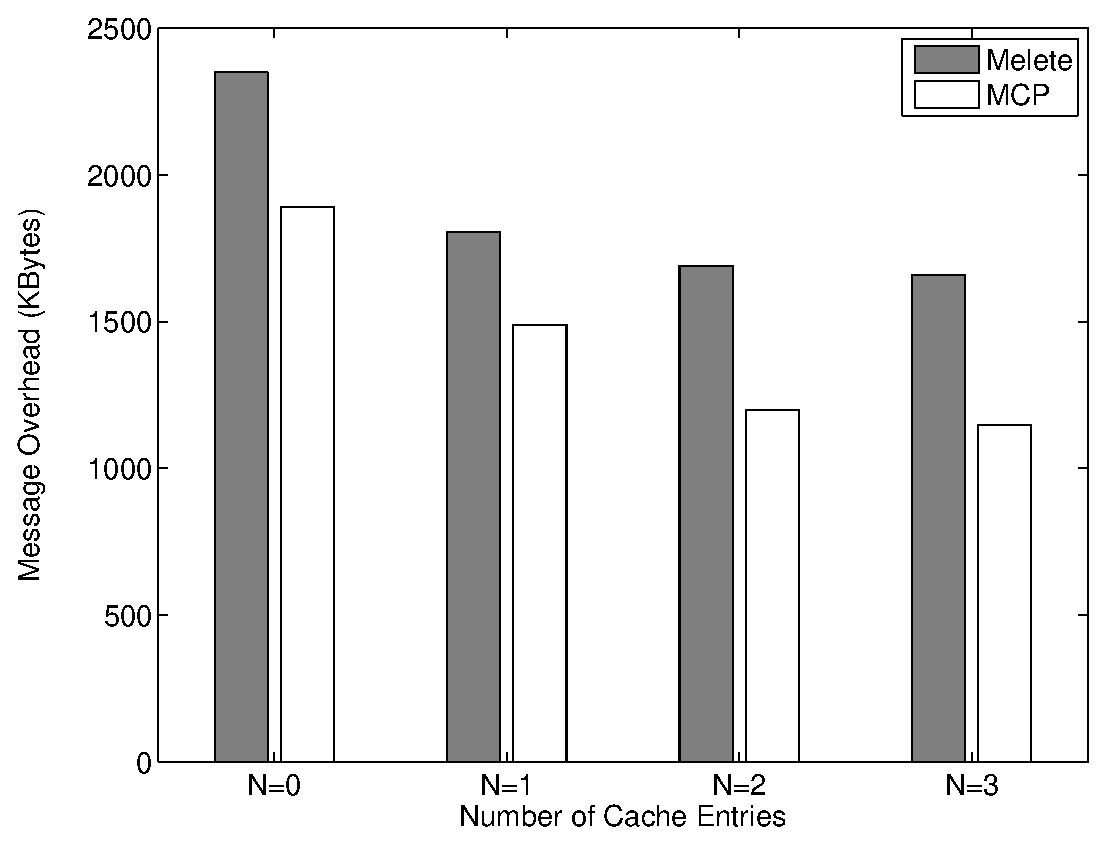
\includegraphics[width=4.2in]{figures/fcache.eps}
\caption{Dissemination with Different Cache Sizes.}
\label{fcache}
\vspace{-0.2in}
\end{figure}


\subsection{Sensitivity to cache sizes}
Fig~\ref{fcache} summarizes message overhead of Melete and MCP with different cache sizes, i.e., the number of code pages that may be cached in memory. Here N=1 denotes that there is no caching. From the figure, MCP achieves significant communication overhead reduction when caching one or two future pages, and diminishing benefits when with larger cache sizes. The reason is that in MCP, a request message can preempt a working node (a source, a requester, or a forwarder) if that node works on a page with a larger page number and the page index difference is bigger than one. In this way, MCP prioritizes slow requesters such that they can keep up the pace with the nearby dissemination and take advantage of cached packets.










